% Completa los datos convenientemente en las zonas marcadas con TODO

\documentclass{beamer}
%PARA VISUALIZAR PRESENTACIONN CON NOTAS USAR VISUALIZADOR "pdfpc":
%Para ver las notas, el cronometro y siguente diapo:
% pdfpc --notes=right slides.pdf
% "tecla p": para pausar el cronometro
\mode<presentation> {
  \usetheme{CambridgeUS}
  \usecolortheme{crane} % color naranja
}
\setbeamercolor{titlelike}{parent=structure,bg=yellow!85!orange} % Cambia el color de la caja del título de la página inicial

\setbeamertemplate{navigation symbols}{} % ocultar iconos de navegación
\setbeamerfont{subsection in toc}{size=\small} % reducir tamaño en TOC
\setbeamerfont{date}{size=\tiny}
\setbeamertemplate{caption}[numbered]



\usepackage[spanish]{babel}
\usepackage[utf8]{inputenc}
\usepackage{graphicx}
\usepackage{booktabs}
\usepackage{hyperref}
\usepackage{multicol}
\usepackage{pgfpages}
\usepackage{listings}
\usepackage{multimedia}
\usepackage[export]{adjustbox}
\usepackage{outlines} % Para poner bullets tabulados (\1 \2 \3 ...) y no items
%Import the natbib package and sets a bibliography  and citation styles
\usepackage[numbers]{natbib}
\usepackage{breakcites}

%\setcitestyle{authoryear,open={((},close={))}} %Citation-related commands

\usepackage{array,tabularx} % para tabular leyenda de ecuaciones
\newenvironment{conditions*} % entorno de "leyenda de ecuación"
  {\par\vspace{\abovedisplayskip}\noindent
   \tabularx{\columnwidth}{>{$}l<{$} @{\ : } >{\raggedright\arraybackslash}X}}
  {\endtabularx\par\vspace{\belowdisplayskip}}
  
% USO DE NOTAS
\setbeameroption{hide notes} % Para mostrar u ocultar (hide/show) DESACTIVAR PARA VER NOTAS
%\setbeameroption{show only notes} % Mostrar solo las notas ACTIVAR PARA VER NOTAS
%\setbeameroption{show notes on second screen=right} % Mostrar notas en otra pantalla
%\setbeamertemplate{note page}{ % asi solo muestro el texto de las notas
 % \insertnote%
%}

%========= TODO: datos internos del documento
\hypersetup{
	pdftitle={Defensa de trabajo de fin de master de David Alarcón Rubio},
	pdfauthor={David Alarcón Rubio}
	pdfsubject={Análisis de redes sociales dinámicas de aprendizaje colaborativo},
	pdfkeywords={teaching, robotics, vision, sensors, actuators, raspberry},
	pdfproducer={pdfLaTeX},
  colorlinks=true,
  linkcolor=blue
}
%=========

%========= TODO: diapositiva de portada
\title[Análisis de Redes Sociales Dinámicas]{Análisis de redes sociales dinámicas de aprendizaje colaborativo} % El título reducido aparece en la parte inferior de todas las diapositivas
                                         % El título completo aparece solo en la diapositiva de portada
\author[David Alarcón Rubio]{David Alarcón Rubio}
\institute[UNED]
{
\textit{\href{mailto:dalarcon32@alumno.uned.es}{\color{blue}{\underline{dalarcon32@alumno.uned.es}}}}\\
\vspace{0.5cm}

Trabajo fin del máster de ingeniería y ciencia de datos\\
Universidad Nacional de Educación a Distancia\\
\vspace{0.5cm}

\includegraphics[width=3cm]{figs/LogoUNED.png}\\
\vspace{0.5cm}
Director: Antonio Rodríguez Anaya
}
\date{29 de junio de 2023}
%=========

%========= COMIENZO DEL DOCUMENTO
\begin{document}

%========= Portada inicial con notas
\begin{frame}[plain] % plain: quita header y footer
\large{\titlepage}
\note[item]{
\begin{itemize}
	\item mis notas para ver como va
	\item mas notasllllllllllllllllllllllllllllll
\end{itemize}

}
\note[item]{En primer lugar...}
\end{frame}

%%========= Licencia
%\begin{frame}
%% Este diseño se corresponde con la licencia CC-BY-NC-SA.
% Por supuesto, puedes poner la licencia que mejor se adapte al propósito de tu trabajo.
% Recuerda que, si no se especifica ninguna licencia, esta -como cualquier creación artística- pasaría a estar licenciada con todos los derechos reservados (copyright).

\vspace{5cm}

\begin{flushright}

\begin{figure}

\includegraphics[width=0.10\textwidth,right]{figs/by-nc-sa.png}
\end{figure}

\vspace{0.2cm}

{\tiny 
(CC) \textbf{Julio Vega}\\ % TODO: pon aquí tu nombre cuando hagas el documento
\vspace{0.5cm}
\emph{
Este trabajo se entrega bajo licencia \href{https://creativecommons.org/licenses/by-nc-sa/3.0/es/}{CC BY-NC-SA}. \\
Usted es libre de \textit{(a) compartir}: copiar y redistribuir el material en \\
cualquier medio o formato; y \textit{(b) adaptar}: remezclar, transformar \\
y crear a partir del material. El licenciador no puede revocar estas \\
libertades mientras cumpla con los términos de la licencia. \\}
}

\end{flushright}


%\end{frame}

%========= Índice o tabla de contenidos (TOC)
\begin{frame}
\frametitle{Contenidos}
%\begin{multicols}{2} % si tengo muchas secciones, lo parte en dos columnas
  \tableofcontents[hideallsubsections] % no muestra subsecciones
%\end{multicols}
\note[item]{La presentaci\'on esta dividida en cuatro partes}
\end{frame}


\section{Introducción}
\subsection{Contexto general}

%========= Diapositiva con ítems resaltados con colores:
\begin{frame}
	\frametitle{Aprendizaje colaborativo}
	\begin{itemize}
		\item En un mundo cada vez más conectado, el aprendizaje colaborativo online se ha convertido en una herramienta poderosa para adquirir conocimientos y desarrollar habilidades \citep{marcos_learning_2019}. 
		\item  Las redes sociales de aprendizaje virtual se convierten en espacios donde los estudiantes pueden interactuar, colaborar y aprender unos de otros \citep{soleymani_using_2022}. 
		\item  Los foros de una asignatura son mucho más que simples espacios para hacer preguntas y respuestas. Son entornos sociales dinámicos donde los estudiantes construyen conocimiento juntos \citep{karina_social_2015}.
		\item  El análisis de redes sociales aplicado a los foros proporciona información valiosa sobre la participación de los estudiantes, lo que puede ser utilizado para monitorear su progreso de aprendizaje y predecir su rendimiento académico \citep{romero2013a,froehlich_social_2018}.
	\end{itemize}
\end{frame}


%========= Diapositiva con ítems resaltados con colores:
\begin{frame}
	\frametitle{Pregunta de investigación y motivación del estudio}
	\begin{block}{¿Cómo podemos utilizar el análisis de redes sociales de aprendizaje colaborativo para predecir el abandono de los estudiantes?}
	En el ámbito educativo, el análisis de \textcolor{red}{redes sociales} y el \textcolor{blue}{aprendizaje automático} pueden ser herramientas poderosas para comprender las interacciones entre los estudiantes y predecir el \textcolor{olive}{abandono de asignaturas}. 
	\end{block}
	\begin{block}{Motivación del estudio}
	\begin{itemize}
	\item  Analizar las interacciones y la estructura social en una comunidad educativa en línea utilizando técnicas de análisis de redes sociales aplicadas a los foros de discusión de una asignatura.
	\item  Desarrollar modelos de aprendizaje automático supervisado para predecir el abandono de los estudiantes en una asignatura, utilizando medidas de centralidad de la red social y medidas del sentimiento expresado en los mensajes.
	\end{itemize}. 
	\end{block}
\end{frame}

\subsection{Estado del arte}


\section{Objetivos}
\subsection{Objetivos principales}
%========= Diapositiva con ítems resaltados con colores:
\begin{frame}
	\frametitle{Objetivos principales}
	\begin{block}{Objetivo Principal: Evaluar la eficacia del análisis de redes sociales dinámicas en la predicción del abandono estudiantil en una asignatura.}
		\begin{itemize}
			\item  Objetivo 1: Analizar la eficacia de las predicciones basadas en el análisis de redes sociales, considerando diferentes rangos de tiempo desde el inicio del curso.
					
			\item  Objetivo 2: Evaluar la eficacia del análisis de las redes temporales al subdividir el rango temporal en bloques de días seriados secuencialmente.
			
			\item  	Objetivo 3: Evaluar la eficacia del análisis de las redes temporales dinámicas al analizar bloques seriados dinámicamente o encadenados.
					
		\end{itemize}. 
	\end{block}
\end{frame}

\subsection{Operativización de los objetivos principales}
%========= Diapositiva con ítems resaltados con colores:
\begin{frame}
	\frametitle{Rangos de tiempo}
	Se analizaron cuatro rangos de tiempo: 30, 60, 90 y 120 días. Estos rangos representan segmentos específicos de interacción en los foros de los estudiantes desde el inicio del curso. 
	\begin{table}[H]
		\centering
		\begin{tabular}{rr}
			\toprule
			Rangos de tiempo & Porcentaje de cobertura \\
			\midrule
			30 días & 25\% \\
			60 días & 50\% \\
			90 días & 75\% \\
			120 días & 100\% \\
			\bottomrule
		\end{tabular}
		\caption{Porcentaje de cobertura por rango de tiempo.}
		\label{tab:subdivision-porcentaje1}
	\end{table}
\end{frame}

%========= Diapositiva con ítems resaltados con colores:
\begin{frame}
	\frametitle{Rangos de tiempo}
	\begin{figure}
		\centering
		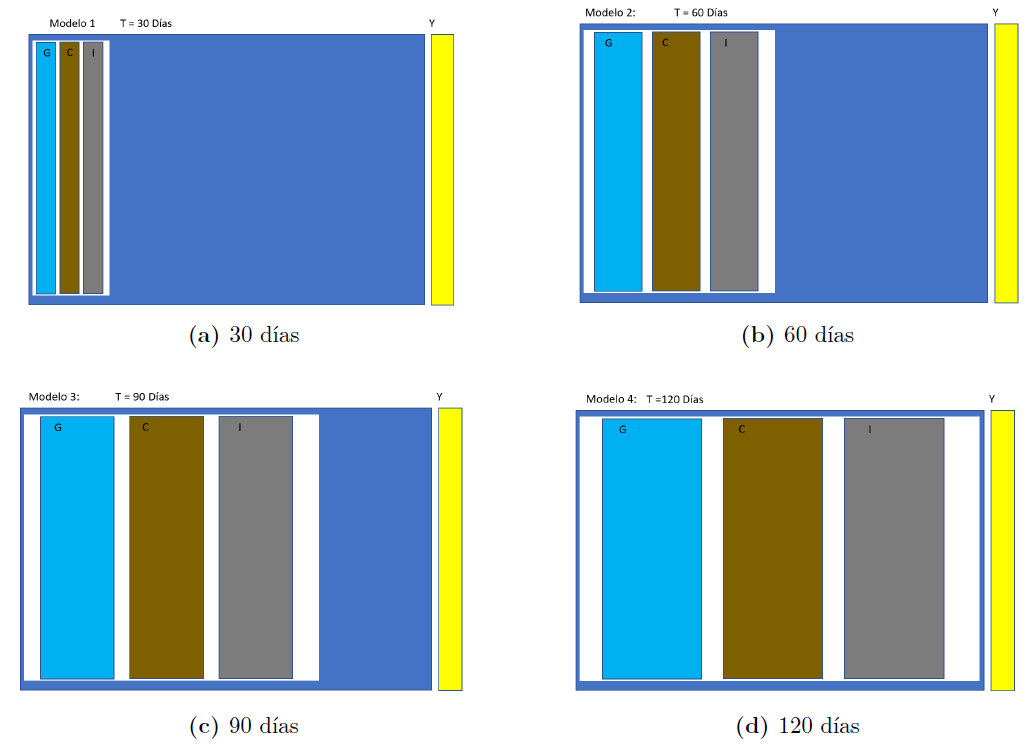
\includegraphics[width=0.7\linewidth]{figs/fig1}
		\caption{Evaluación de la eficacia de lso diferentes rangos de tiempo en la predicción del abandono}
		\label{fig:fig1}
	\end{figure}
\end{frame}


%========= Diapositiva con ítems resaltados con colores:
\begin{frame}
	\frametitle{Subdivisión en bloques}
	La subdivisión en bloques permite un análisis más detallado de la red social en segmentos específicos de tiempo \citep{kim2012a}. Se consideraron diferentes rangos temporales y se determinaron las opciones de subdivisión en bloques. 
	\begin{table}[H]
		\centering
		\begin{tabular}{ll}
			\toprule
			Rangos & Número de días $\times$ Número de bloques \\
			\midrule
			30 días & 5 $\times$ 6, 10 $\times$ 3, 15 $\times$ 2 \\
			60 días & 5 $\times$ 12, 10 $\times$ 6, 15 $\times$ 4, 20 $\times$ 3, 30 $\times$ 2 \\
			90 días & 5 $\times$ 18, 10 $\times$ 9, 15 $\times$ 6, 30 $\times$ 3, 45 $\times$ 2 \\
			120 días & 5 $\times$ 24, 10 $\times$ 12, 15 $\times$ 8, 20 $\times$ 6, 30 $\times$ 4, 40 $\times$ 3, 60 $\times$ 2 \\
			\bottomrule
		\end{tabular}
		\caption{Opciones de subdivisión en bloques para cada rango temporal.}
		
		\label{tab:subdivision-bloques1}
	\end{table}

\end{frame}


%========= Diapositiva con ítems resaltados con colores:
\begin{frame}
	\frametitle{Subdivisión en bloques seriados secuencialmente}
	\begin{figure}
		\centering
		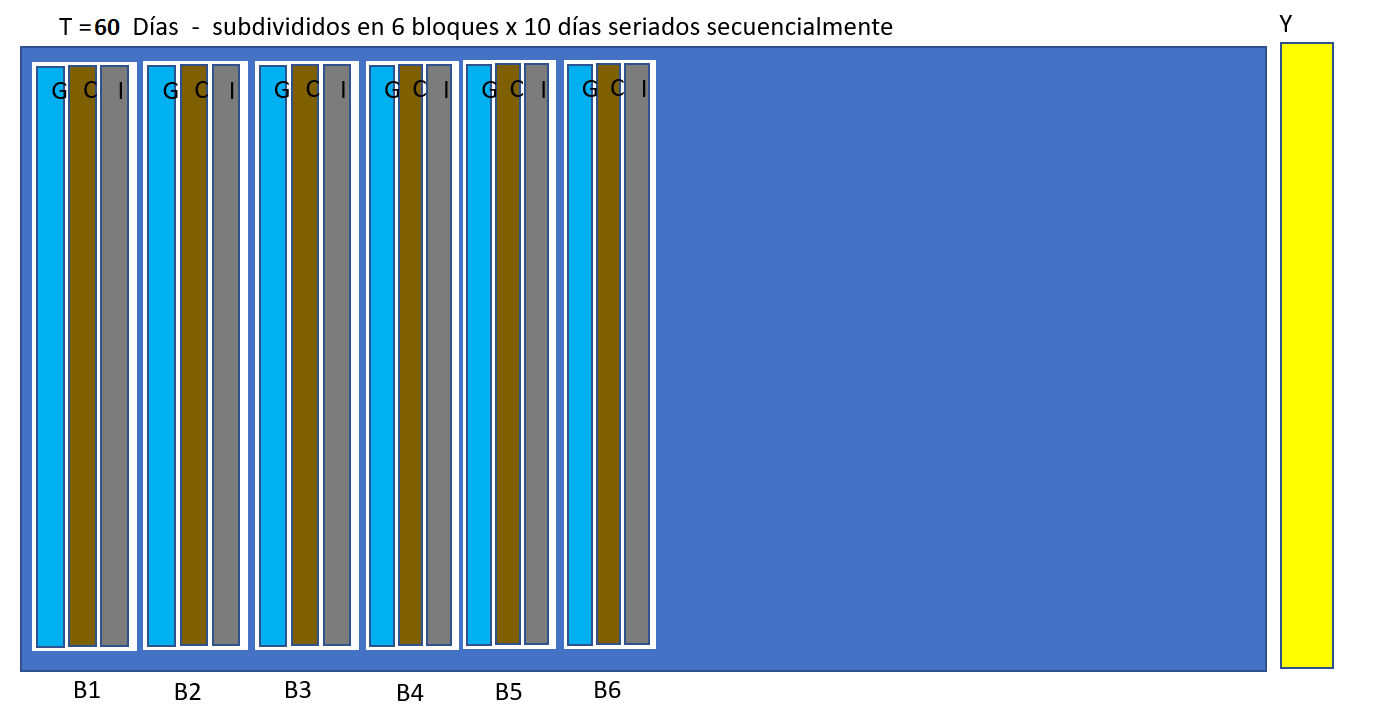
\includegraphics[width=0.7\linewidth]{figs/imagen20}
		\caption{Subdivisión del rango de tiempo en bloques seriados secuencialmente}
		\label{fig:imagen320}
	\end{figure}
	
\end{frame}


%========= Diapositiva con ítems resaltados con colores:
\begin{frame}
	\frametitle{Subdivisión en bloques dinámicos o encadenados}
	\begin{itemize}
		\item La subdivisión en bloques secuenciales permite analizar las interacciones y dinámicas dentro de cada bloque. La subdivisión en bloques dinámicos o encadenados establece una relación de continuidad entre los bloques, capturando la evolución y los cambios a largo plazo \citep{Mahmoud_2021}.
		\item En la subdivisión en bloques encadenados, cada bloque temporal se superpone con el bloque anterior y el bloque siguiente. 
		\item Esto significa que se comparten nodos y conexiones entre bloques adyacentes, lo que permite capturar la continuidad y los cambios graduales en la red a lo largo del tiempo.
	\end{itemize}	
\end{frame}

%========= Diapositiva con ítems resaltados con colores:
\begin{frame}
	\frametitle{Subdivisión en bloques dinámicos o encadenados}
	\begin{figure}[H]
		\centering
		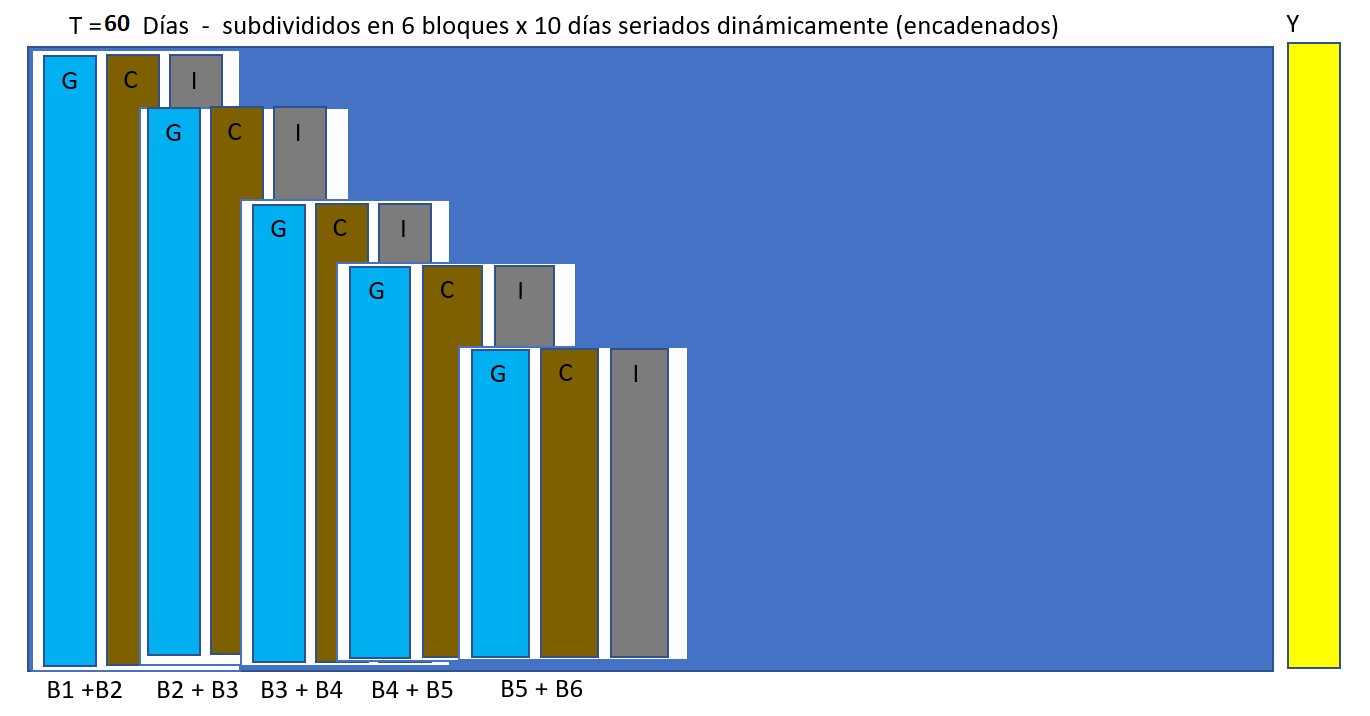
\includegraphics[width=0.7\linewidth]{figs/imagen21}
		\caption{Subdivisión del rango de tiempo en bloques seriados dinámicamente (encadenados)}
		\label{fig:imagen321}
	\end{figure}
	
\end{frame}





\subsection{Atributos}

\begin{frame}
	\frametitle{Medidas de Centralidad en Redes Sociales}
	
	\begin{itemize}
		\item \textbf{Grado (Degree)}: Número de enlaces que tiene un nodo. Los nodos con un alto grado son actores clave para la comunicación y difusión de información.
		
		\item \textbf{Cercanía (Closeness)}: Evalúa la distancia promedio entre un nodo y todos los demás nodos de la red. Los nodos con alta cercanía están más cerca de los demás nodos y pueden acceder rápidamente a la información y difundirla eficientemente.
		
		\item \textbf{Intermediación (Betweenness)}: Se enfoca en los caminos más cortos de la red. Un nodo con alta intermediación se encuentra en muchos caminos más cortos entre otros nodos, actuando como intermediario en la comunicación y transferencia de información en la red.
	\end{itemize}
	
\end{frame}


\begin{frame}
	\frametitle{Medidas de Centralidad en Redes Sociales}
	
	\begin{block}{Medidas de Centralidad Ponderadas}
		\begin{enumerate}
			\item Las medidas de centralidad sin pesos consideran solo la topología de la red.
			\item Las medidas de centralidad con pesos tienen en cuenta los pesos asociados a las conexiones \citep{tang2010a, barrat2004a} .
		\end{enumerate}
	\end{block}
	
	\begin{block}{Medidas de Centralidad Locales o Globales}
		\begin{enumerate}
			\item Las medidas de centralidad local se centran en la importancia de un nodo en relación con sus vecinos directos en la red.
			\item Las medidas de centralidad global (híbridas) evalúan la importancia de los nodos considerando tanto las interacciones directas del nodo como las interacciones de los nodos vecinos a los que está conectado \citep{abbasi2013a, Mahmoud_2021}.
		\end{enumerate}
	\end{block}
	
\end{frame}



\begin{frame}
	\frametitle{Medidas de Sentimiento y Emoción}
	\begin{block}{Sentimiento}
		\begin{itemize}
			\item Métrica utilizada para evaluar el tono emocional transmitido en los mensajes de texto. Asigna un valor numérico entre 0 y 1 representando la probabilidad de que el texto sea "positivo".
		\end{itemize}
	\end{block}
	
	\begin{block}{Russel Valence y Russel Arousal}
		\begin{itemize}
			\item Russel Valence: Métrica que evalúa la carga emocional o la valencia de un texto.
			\item Russel Arousal: Métrica que evalúa el nivel de excitación o activación emocional transmitido por un texto.
		\end{itemize}
	\end{block}
	
	\begin{block}{Emoción}
		\begin{itemize}
			\item Utiliza una región de Russel para clasificar el texto en categorías emocionales como neutro, relajado, feliz, triste o enfadado.
		\end{itemize}
	\end{block}
	
\end{frame}


\section{Subobjetivos e hipótesis}
%========= Diapositiva con ítems resaltados con colores:
\begin{frame}
	\frametitle{Subbjetivos e hipótesis}
	\begin{block}{Subobjetivo 1: Teoría del capital social de la red}
		Hipótesis A: Las medidas de centralidad ponderadas serán más capaces de capturar la importancia de las interacciones entre los nodos y predecir el abandono estudiantil \citep{wasko_why_2005}.
		
	\end{block}
	\begin{block}{Subobjetivo 2: Teoría de la estructura social de la red}
		Hipótesis B: Los modelos de medidas de centralidad globales serán más eficaces para predecir el abandono estudiantil en comparación con los modelos que solo consideran medidas locales \citep{krause_social_2007}.
		
	\end{block}
	\begin{block}{Subobjetivo 3: Teoría del balance social de la red}
		Hipótesis C: Las medidas de centralidad junto a las medidas de sentimiento expresadas en los mensajes podrán predecir el abandono estudiantil de manera más precisa \citep{kim2012a}.
	\end{block}
\end{frame}


%========= Diapositiva con ítems resaltados con colores:
\begin{frame}
	\frametitle{Algoritmos de aprendizaje supervisado}
	
	\begin{itemize}
		\item Regresión Logística: Clasificación binaria basada en un modelo logístico.
		\item SVM (Support Vector Machine): Clasificación y regresión basada en hiperplanos óptimos en un espacio de alta dimensionalidad.
		\item Decision Tree Classifier: Toma de decisiones basada en una estructura de árbol que divide los datos según características.
		\item KNN (K-Nearest Neighbors): Clasificación basada en los K puntos de entrenamiento más cercanos en función de la distancia.
		\item MLP Classifier (Multi-Layer Perceptron): Clasificación basada en redes neuronales artificiales con múltiples capas de nodos.
	\end{itemize}
	
\end{frame}


\begin{frame}
	\frametitle{Métricas de evaluación de la predicción}
	\begin{itemize}
		\item Precisión (Accuracy): Proporción de predicciones correctas sobre el total de predicciones realizadas.
		\item Precisión (Precision): Proporción de verdaderos positivos sobre el total de positivos predichos. Indica qué tan bien el modelo identifica correctamente los casos positivos.
		\item Exhaustividad (Recall): Proporción de verdaderos positivos sobre el total de positivos reales. Indica qué tan bien el modelo captura todos los casos positivos.
		\item Puntuación F1 (F1 Score): Media armónica de la precisión y la exhaustividad. Proporciona una medida equilibrada del rendimiento del modelo.
		\item ROC AUC (Area Under the Receiver Operating Characteristic Curve): Capacidad de discriminación del modelo y su habilidad para distinguir entre las clases positiva y negativa.
	\end{itemize}
	
\end{frame}


\section{Procesamiento de datos y técnicas  de aprendizaje supervisado}
%========= Diapositiva con ítems resaltados con colores:
\begin{frame}
	\frametitle{Modelos predictivos por combinación de factores}
	
	\begin{figure}[H]
		\centering
		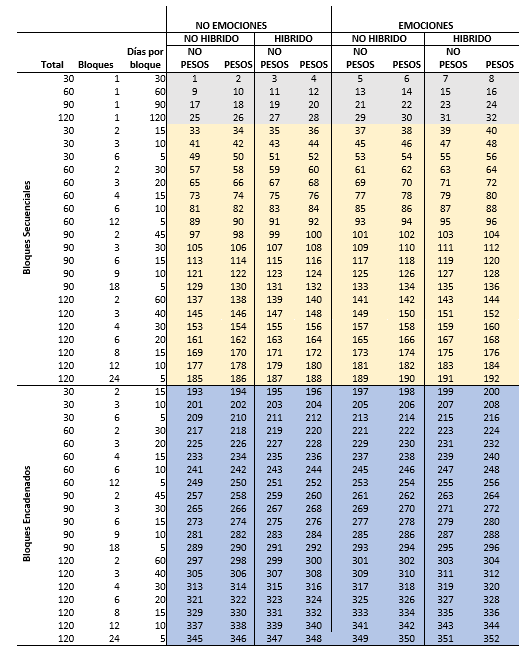
\includegraphics[width=0.5\linewidth]{figs/imagen32}
		\caption{Modelos predictivos por combinación de factores.}
		\label{fig:imagen32}
	\end{figure}
\end{frame}


\begin{frame}
	\frametitle{Índices de evaluación de las redes sociales dinámicas en la predicción}
	\begin{block}{Evaluamos las teorías e hipótesis propuestas utilizando índices construidos específicos.}
	\begin{itemize}
		\item Índice de amplitud o cobertura de la información: mide la proporción del tiempo total de la asignatura cubierta por cada rango de tiempo analizado en los foros de los estudiantes.
		%Mide la capacidad del algoritmo para capturar la diversidad de interacciones en la red social dinámica.
		\item Índice de unidad de información: evalúa el grado de subdivisión en bloques que se utiliza para obtener las medidas de posición de los estudiantes y de expresión de sentimientos.
		%Evalúa la capacidad del algoritmo para identificar grupos o comunidades dentro de la red social dinámica.
		\item Índice de cantidad de información: es una medida que combina el grado de subdivisión en bloques y la proporción de cobertura temporal en el análisis de redes sociales.
		%Cuantifica la cantidad de información relevante proporcionada por el algoritmo sobre las interacciones en la red social dinámica.
	\end{itemize}
	\end{block}
\end{frame}



\section{Resultados}

%========= Diapositiva con ítems resaltados con colores:
\begin{frame}
	\frametitle{Resumen teorías, hipótesis e índices}
	
	\begin{figure}[H]
		\centering
		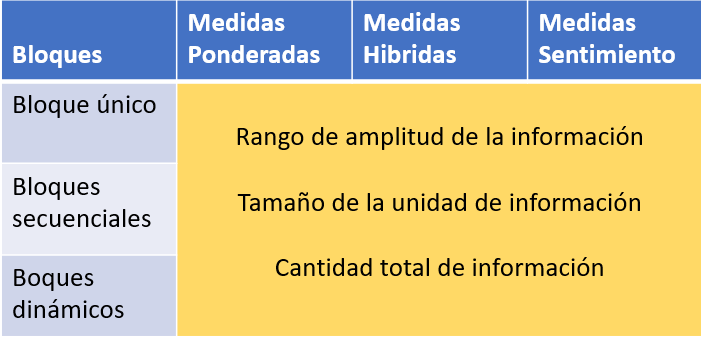
\includegraphics[width=0.9\linewidth]{figs/imagen23}
		\caption{Resumen de teorías, hipótesis e índices}
		\label{fig:imagen23}
	\end{figure}
\end{frame}

\subsection{Objetivos 1, 2 y 3 - Hipótesis A: medidas ponderadas}
%========= Diapositiva con ítems resaltados con colores:
\begin{frame}
	\frametitle{Resultados. Objetivo 1 - Hipótesis A}
	\begin{block}{Objetivo 1. Analizar la eficacia de las predicciones utilizando distintos rangos de tiempo (en un solo bloque).}
		Hipótesis A: medidas de centralidad ponderadas (con pesos vs sin pesos).
	\end{block}
	
\begin{figure}[H]
	\centering
	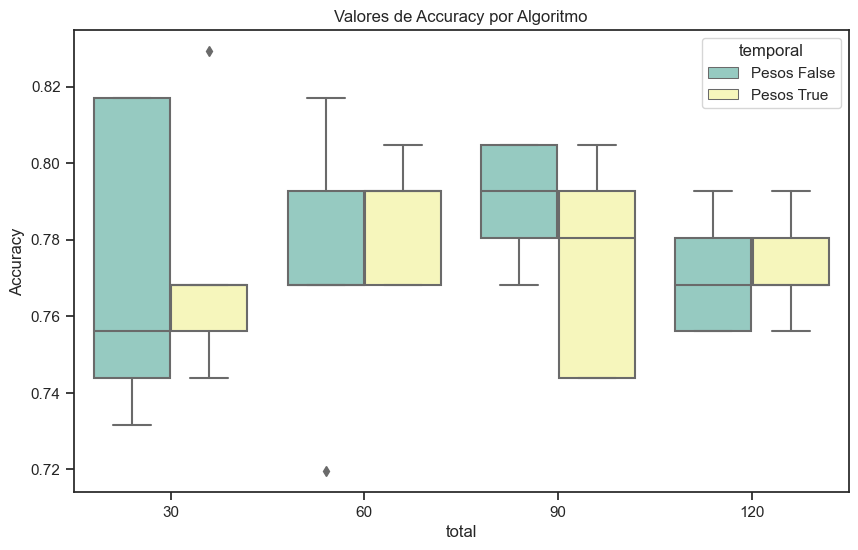
\includegraphics[width=0.7\linewidth]{figs/cap6/figura_12}
	\caption{Gráfico de cajas que compara los valores de Accuracy según el rango de días analizados y el tipo de medida de centralidad (con pesos o sin pesos).}
	\label{fig:figura12}
\end{figure}
	
\end{frame}

%========= Diapositiva con ítems resaltados con colores:
\begin{frame}
	\frametitle{Resultados. Objetivo 2 - Hipótesis A}
	\begin{block}{Objetivo 2. Analizar la eficacia de las predicciones utilizando distintos rangos de tiempo subdivididos por bloques secuenciales.}
		Hipótesis A: medidas de centralidad ponderadas (con pesos vs sin pesos).
	\end{block}
	
\begin{figure}[H]
	\centering
	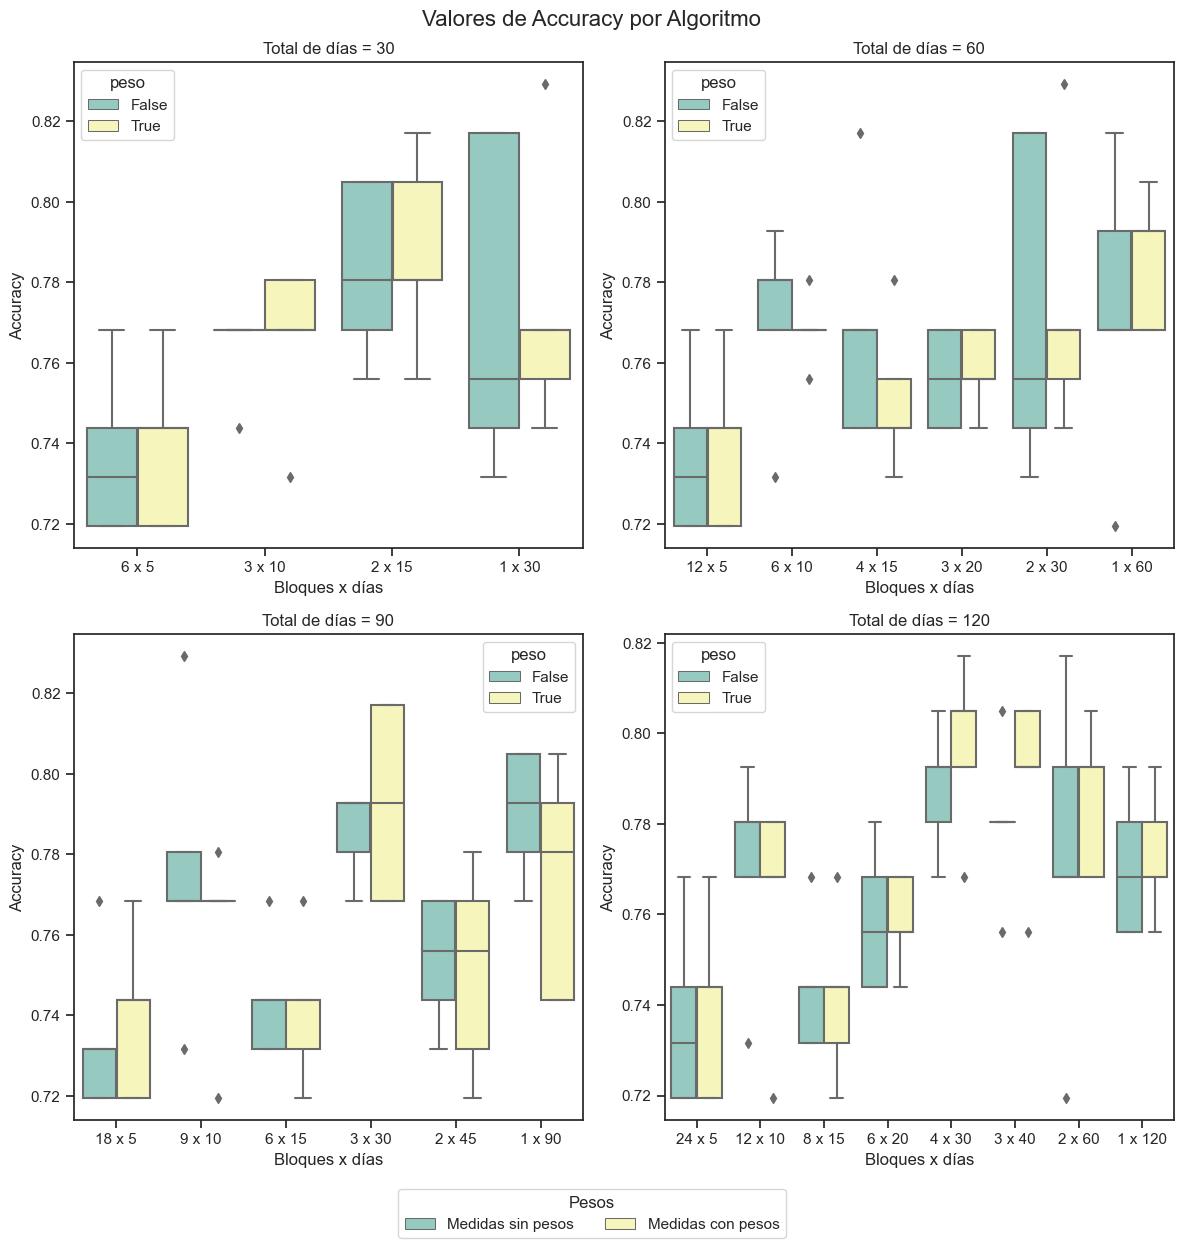
\includegraphics[width=0.45\linewidth]{figs/cap6/figura_26}
	\caption{Comparación de métricas de Accuracy según rango de tiempo y subdivisión en bloques.}
	\label{fig:figura45}
\end{figure}
	
\end{frame}

%========= Diapositiva con ítems resaltados con colores:
\begin{frame}
	\frametitle{Resultados. Objetivo 3 - Hipótesis A}
	\begin{block}{Objetivo 3. Analizar la eficacia de las predicciones utilizando distintos rangos de tiempo subdivididos por bloques encadenados.}
		Hipótesis A: medidas de centralidad ponderadas (con pesos vs sin pesos).
	\end{block}
	
\begin{figure}[H]
	\centering
	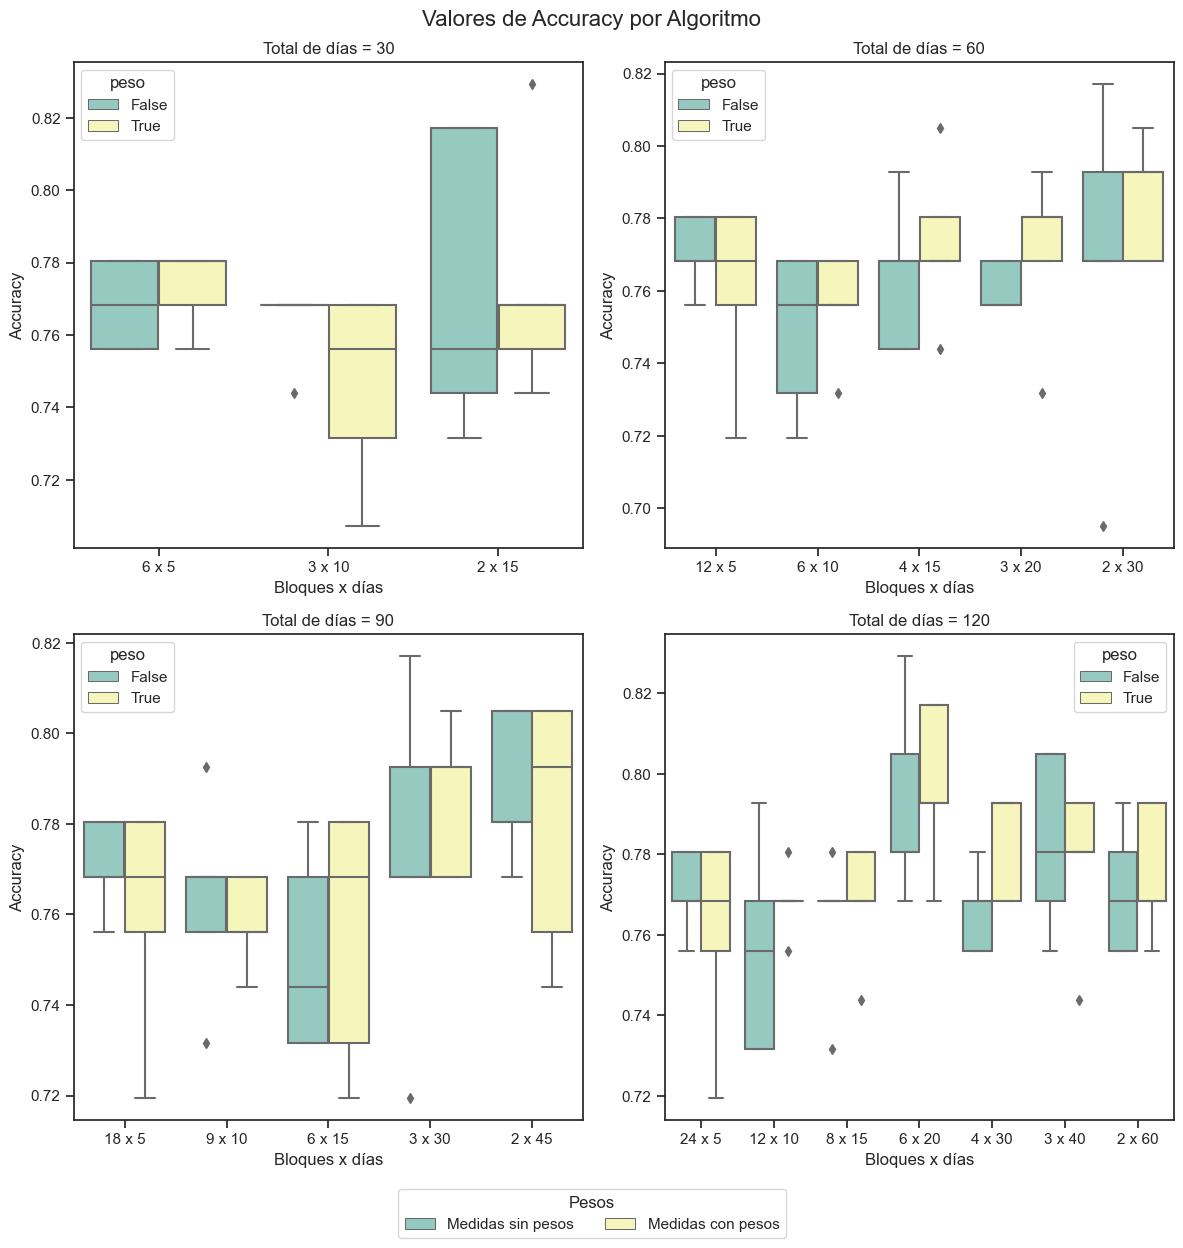
\includegraphics[width=0.45\linewidth]{figs/cap6/figura_84}
	\caption{Variación de Accuracy según los rangos de tiempo analizados y los bloques de días.}
	
	\label{fig:figura84}
\end{figure}

\end{frame}


\subsection{Objetivos 1, 2 y 3 - Hipótesis B: Medidas híbridas}
%========= Diapositiva con ítems resaltados con colores:
\begin{frame}
	\frametitle{Resultados. Objetivo 1 - Hipótesis B}
	\begin{block}{Objetivo 1. Analizar la eficacia de las predicciones utilizando distintos rangos de tiempo (en un solo bloque).}
		Hipótesis B: medidas de centralidad locales vs globales (híbridas).
	\end{block}
	
\begin{figure}[H]
	\centering
	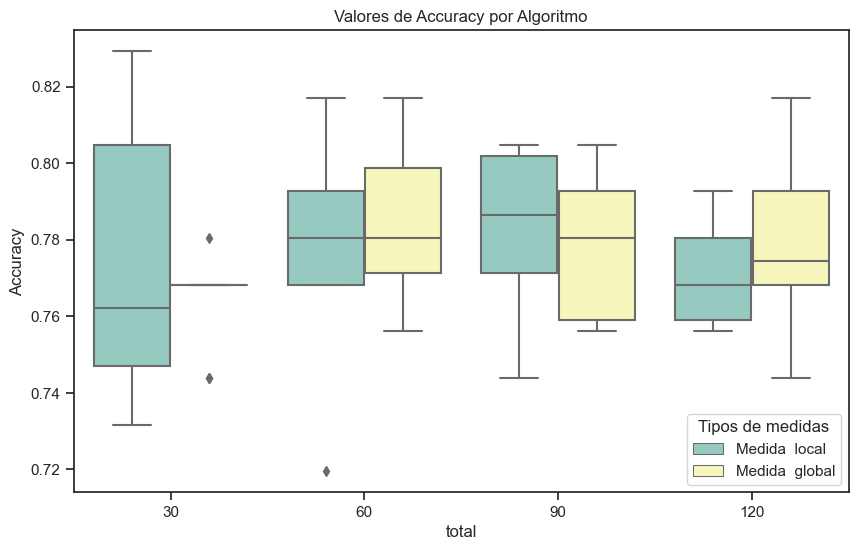
\includegraphics[width=0.7\linewidth]{figs/cap6/figura_24}
	\caption{Comparación de los valores de Accuracy según el tipo de medida de centralidad (local o global).}
	\label{fig:figura24}
\end{figure}
\end{frame}

%========= Diapositiva con ítems resaltados con colores:
\begin{frame}
	\frametitle{Resultados. Objetivo 2 - Hipótesis B}
	\begin{block}{Objetivo 2. Analizar la eficacia de las predicciones utilizando distintos rangos de tiempo subdivididos por bloques secuenciales.}
		Hipótesis B: medidas de centralidad locales vs globales (híbridas).
	\end{block}
	

\begin{figure}[H]
	\centering
	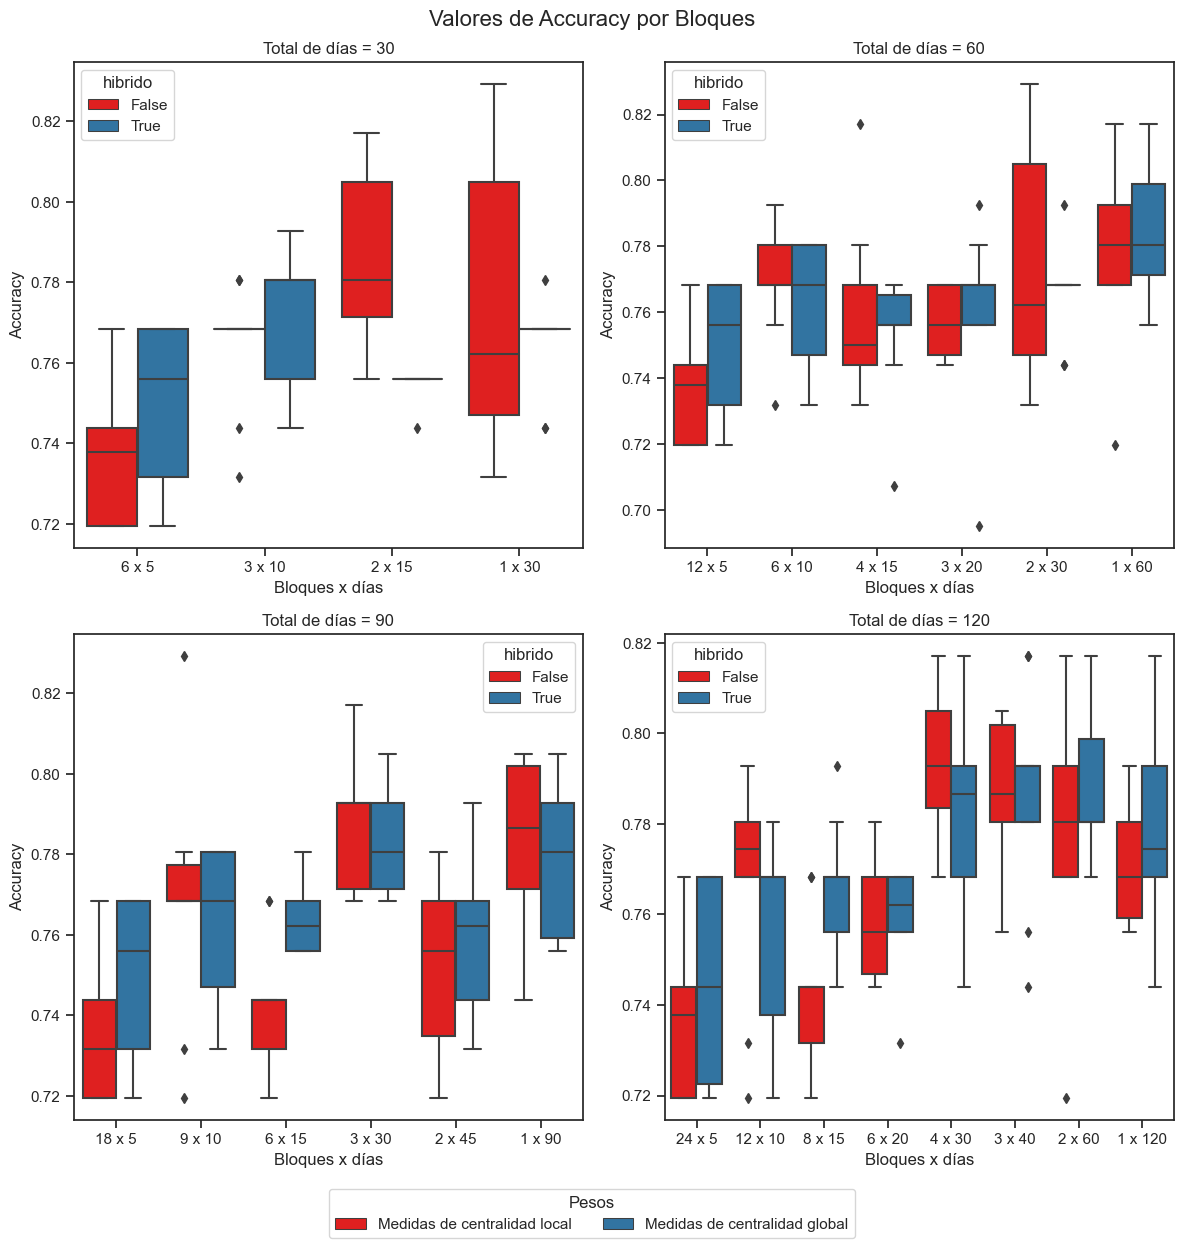
\includegraphics[width=0.45\linewidth]{figs/cap6/figura_47}
	\caption{Variación de Accuracy según rangos de tiempo y medidas de centralidad.}
	
	\label{fig:figura647}
\end{figure}
	
\end{frame}

%========= Diapositiva con ítems resaltados con colores:
\begin{frame}
	\frametitle{Resultados. Objetivo 3 - Hipótesis B}
	\begin{block}{Objetivo 3. Analizar la eficacia de las predicciones utilizando distintos rangos de tiempo subdivididos por bloques encadenados.}
		Hipótesis B: medidas de centralidad locales vs globales (híbridas).
	\end{block}
	

\begin{figure}[H]
	\centering
	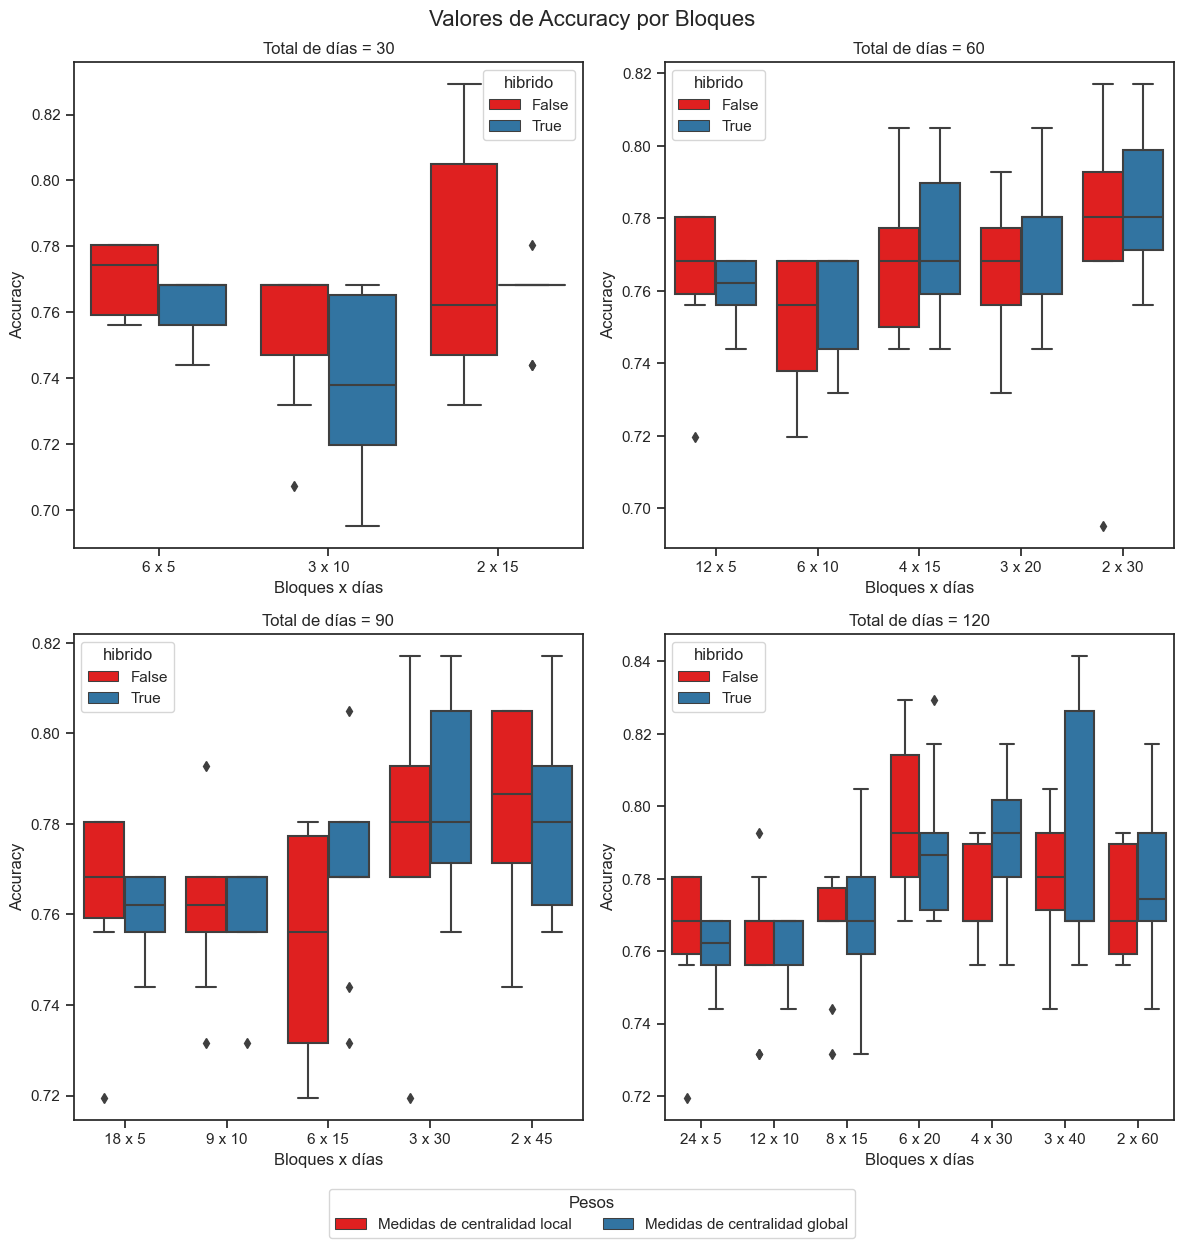
\includegraphics[width=0.45\linewidth]{figs/cap6/figura_105}
	\caption{Variación de Accuracy según rangos de tiempo y medidas de centralidad.}
	
	\label{fig:figura105}
\end{figure}

	
\end{frame}


\subsection{Objetivos 1, 2 y 3 - Hipótesis C: Medidas de sentimiento}
%========= Diapositiva con ítems resaltados con colores:
\begin{frame}
	\frametitle{Resultados. Objetivo 1 - Hipótesis C}
	\begin{block}{Objetivo 1. Analizar la eficacia de las predicciones utilizando distintos rangos de tiempo (en un solo bloque).}
		Hipótesis C: medidas de centralidad vs medidas centralidad-sentimiento.
	\end{block}
	
\begin{figure}[H]
	\centering
	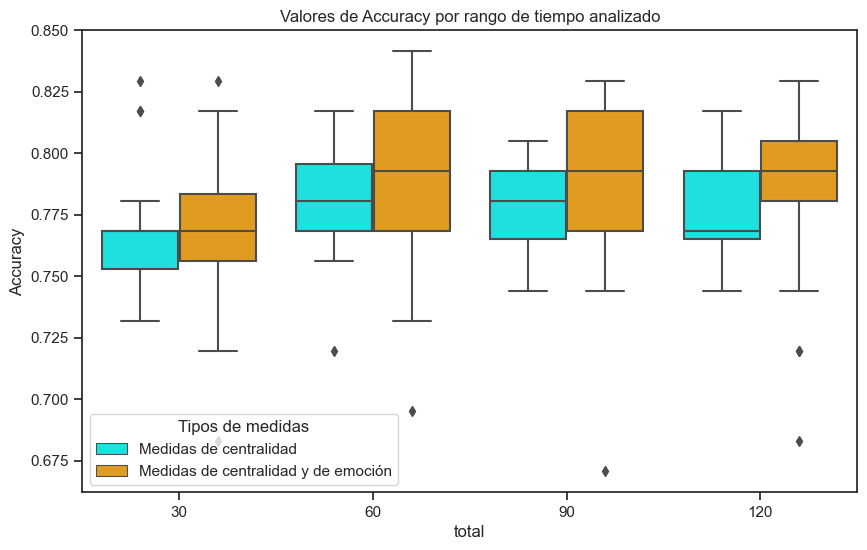
\includegraphics[width=0.7\linewidth]{figs/cap6/figura_32}
	\caption{Comparación de los valores de Accuracy según el rango de tiempo y la consideración de medidas de centralidad y emociones.}
	
	\label{fig:figura33}
\end{figure}


	
\end{frame}

%========= Diapositiva con ítems resaltados con colores:
\begin{frame}
	\frametitle{Resultados. Objetivo 2 - Hipótesis C}
	\begin{block}{Objetivo 2. Analizar la eficacia de las predicciones utilizando distintos rangos de tiempo subdivididos por bloques secuenciales.}
		Hipótesis C: medidas de centralidad vs medidas centralidad-sentimiento.
	\end{block}
	
\begin{figure}[H]
	\centering
	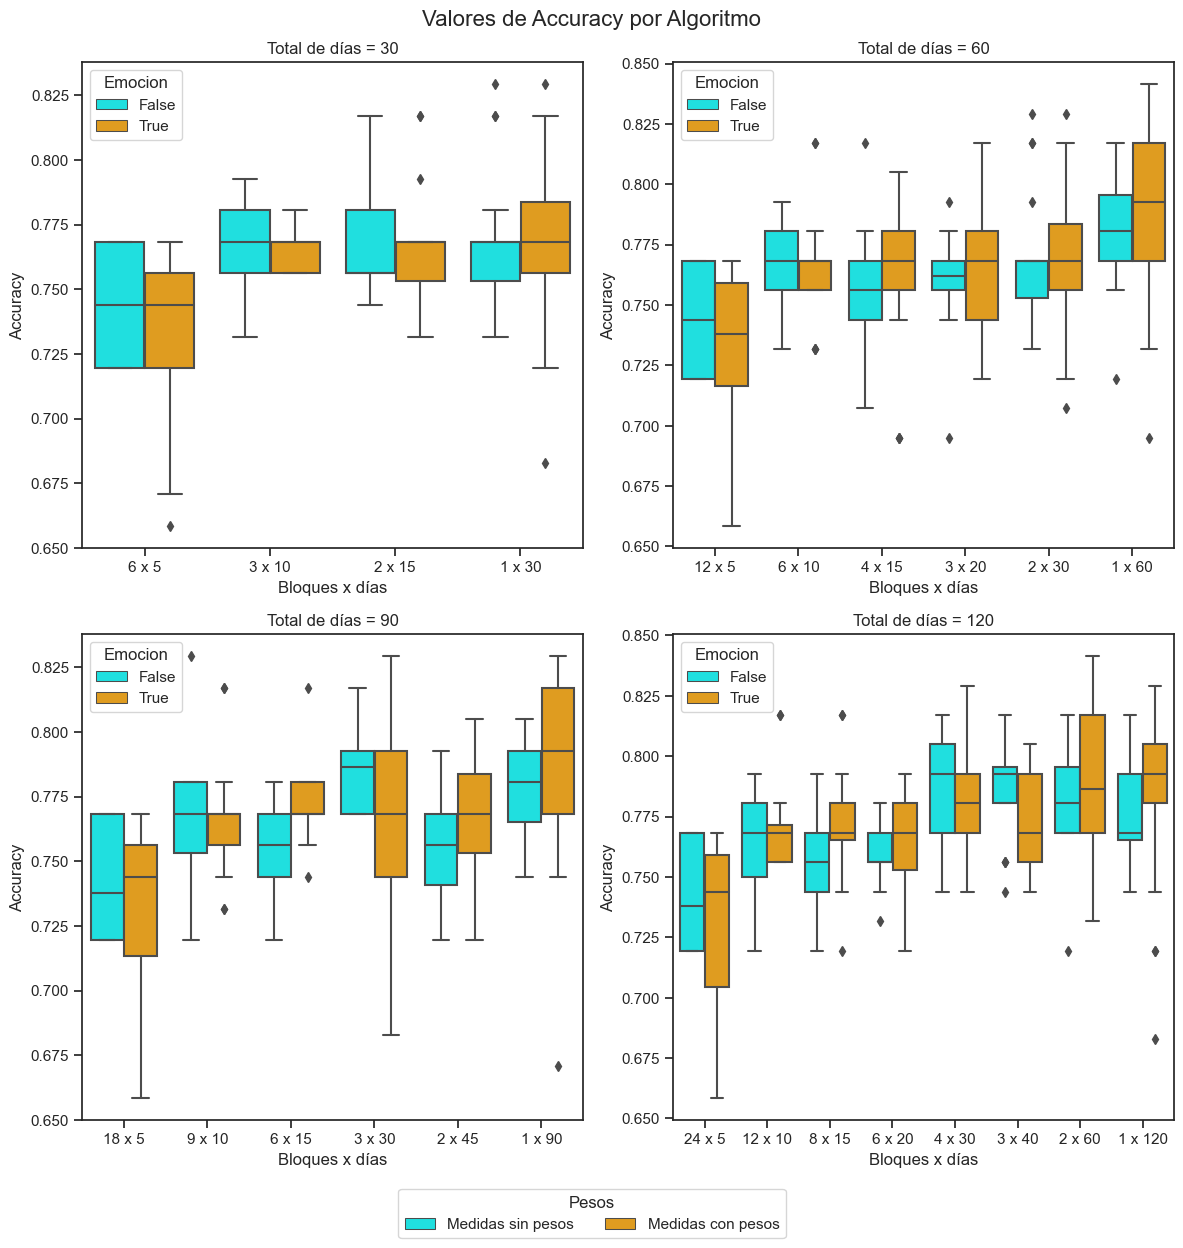
\includegraphics[width=0.45\linewidth]{figs/cap6/figura_64}
	\caption{Métricas de Accuracy en función de los distintos rangos de tiempo analizados y los bloques de días}
	\label{fig:figura58}
\end{figure}


\end{frame}

%========= Diapositiva con ítems resaltados con colores:
\begin{frame}
	\frametitle{Resultados. Objetivo 3 - Hipótesis C}
	\begin{block}{Objetivo 3. Analizar la eficacia de las predicciones utilizando distintos rangos de tiempo subdivididos por bloques encadenados.}
		Hipótesis C: medidas de centralidad vs medidas centralidad-sentimiento.
	\end{block}
	
\begin{figure}[H]
	\centering
	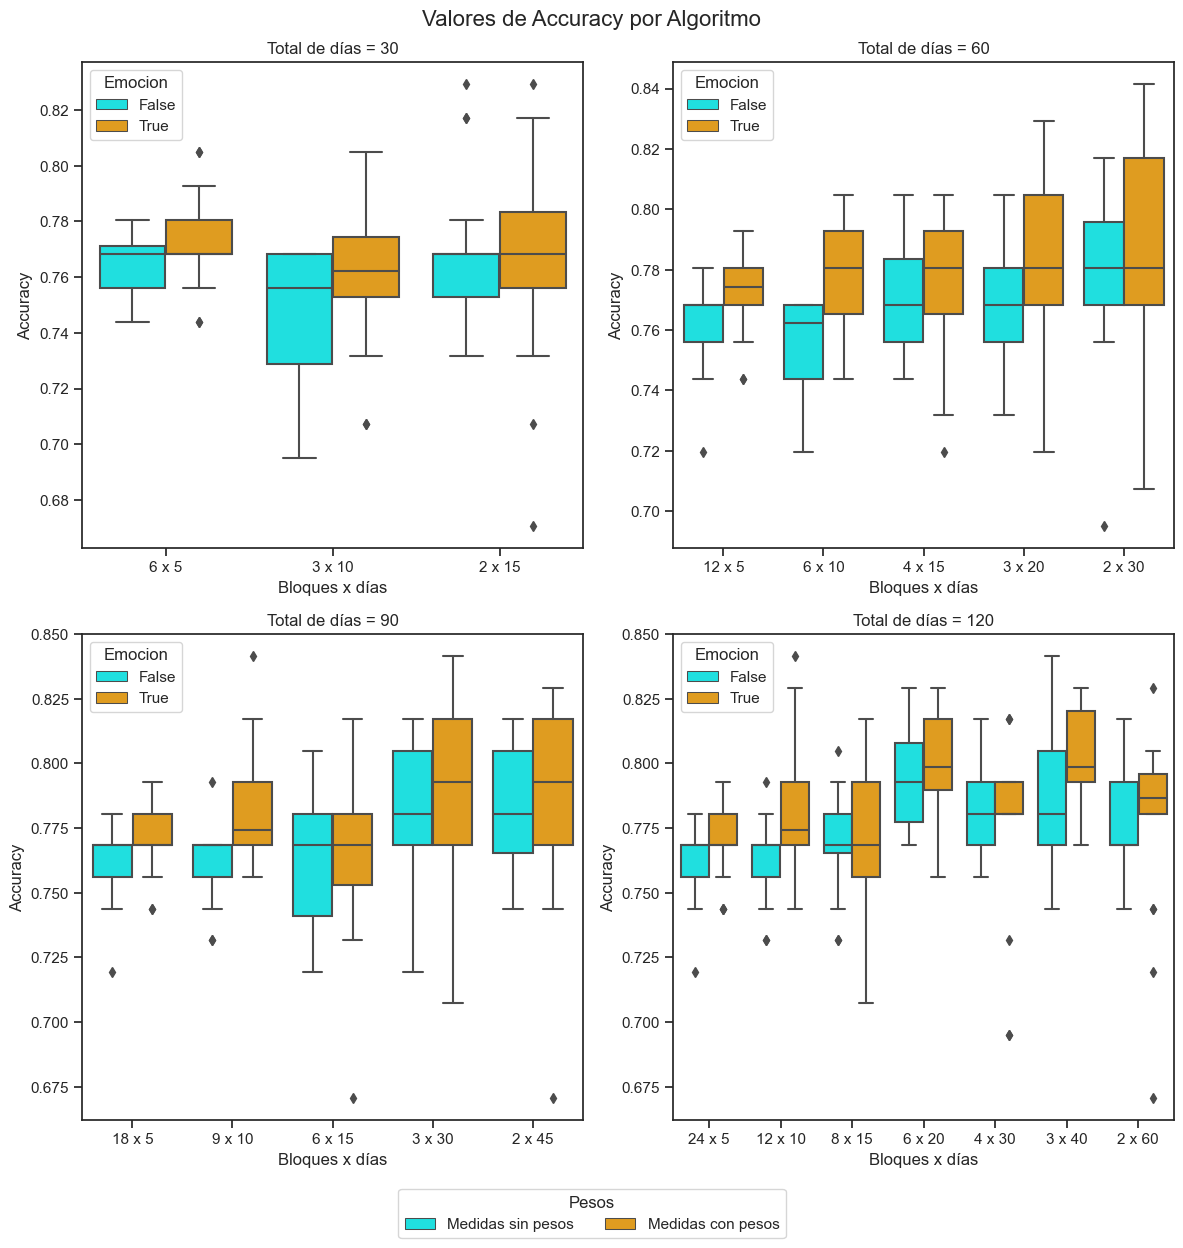
\includegraphics[width=0.45\linewidth]{figs/cap6/figura_122}
	\caption{Accuracy según rangos de tiempo y medidas de centralidad local (sin pesos y con pesos).}
	
	\label{fig:figura121}
\end{figure}

\end{frame}



\subsection{ Objetivo 1 - Rangos Tempolares}
%%========= Diapositiva con ítems resaltados con colores:
\begin{frame}
	\frametitle{Resultados. Objetivo 1 - Rangos Tempolares}
	\begin{block}{Analizar la eficacia de las predicciones utilizando distintos rangos de tiempo en cualquier tipo de subdivisión por bloques (un bloque único, bloques secuenciales y bloques encadenados).}
		Índice de amplitud o cobertura de la información.
	\end{block}
	
\begin{figure}[H]
	\centering
		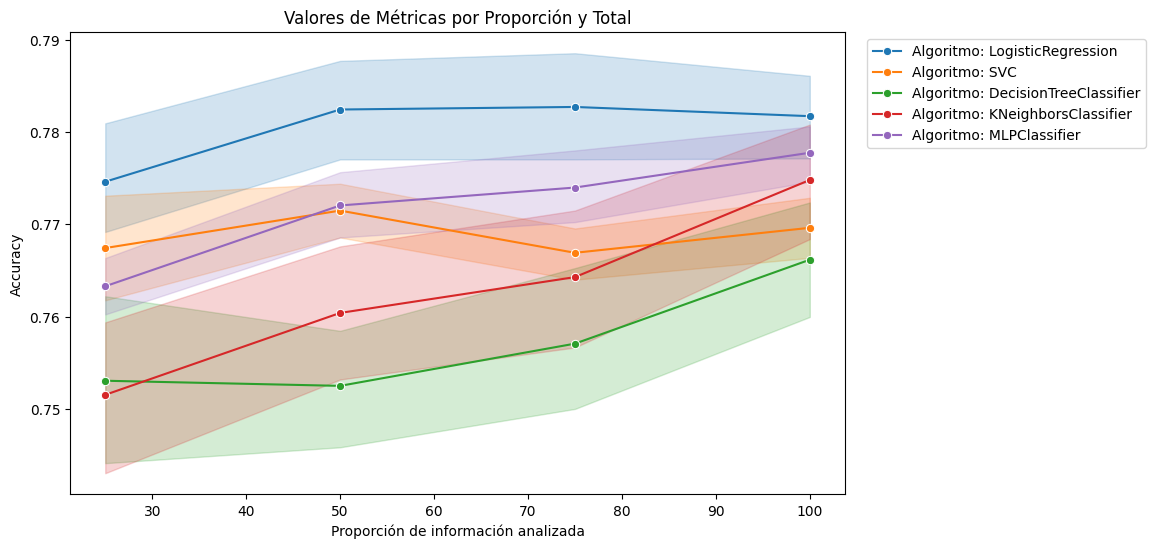
\includegraphics[width=0.6\linewidth]{figs/cap7/figura_14}
	\caption{Eficacia de los algoritmos de aprendizaje supervisado en función del índice de amplitud de información}
	
	\label{fig:figura205}
\end{figure}
	
\end{frame}


%========= Diapositiva con ítems resaltados con colores:
\begin{frame}
	\frametitle{Resultados. Objetivo 1 - Rangos Tempolares}
	\begin{block}{Analizar la eficacia de las predicciones utilizando distintos rangos de tiempo en cualquier tipo de subdivisión por bloques (un bloque único, bloques secuenciales y bloques encadenados).}
		Índice de tamaño de la unidad de información.
	\end{block}
	
\begin{figure}[H]
	\centering
	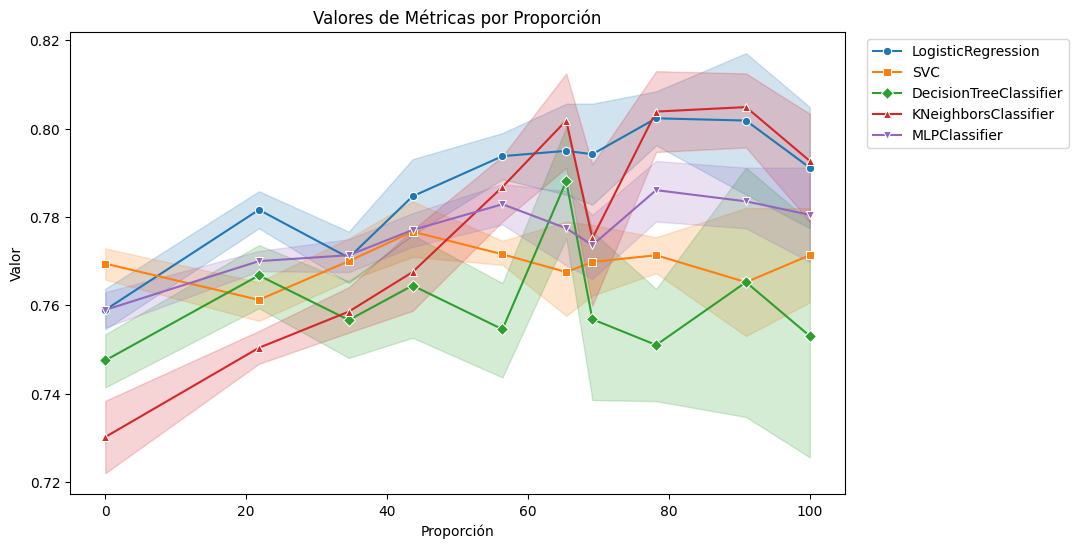
\includegraphics[width=0.6\linewidth]{figs/cap7/figura_12}
	\caption{Eficacia de los algoritmos de aprendizaje supervisado en función del índice de unidad de información}
	
	\label{fig:figura206}
\end{figure}

	
\end{frame}


%========= Diapositiva con ítems resaltados con colores:
\begin{frame}
	\frametitle{Resultados. Objetivo 1 - Rangos Tempolares}
	\begin{block}{Analizar la eficacia de las predicciones utilizando distintos rangos de tiempo en cualquier tipo de subdivisión por bloques (un bloque único, bloques secuenciales y bloques encadenados).}
		Índice de cantidad de información.
	\end{block}
	
\begin{figure}[H]
	\centering
	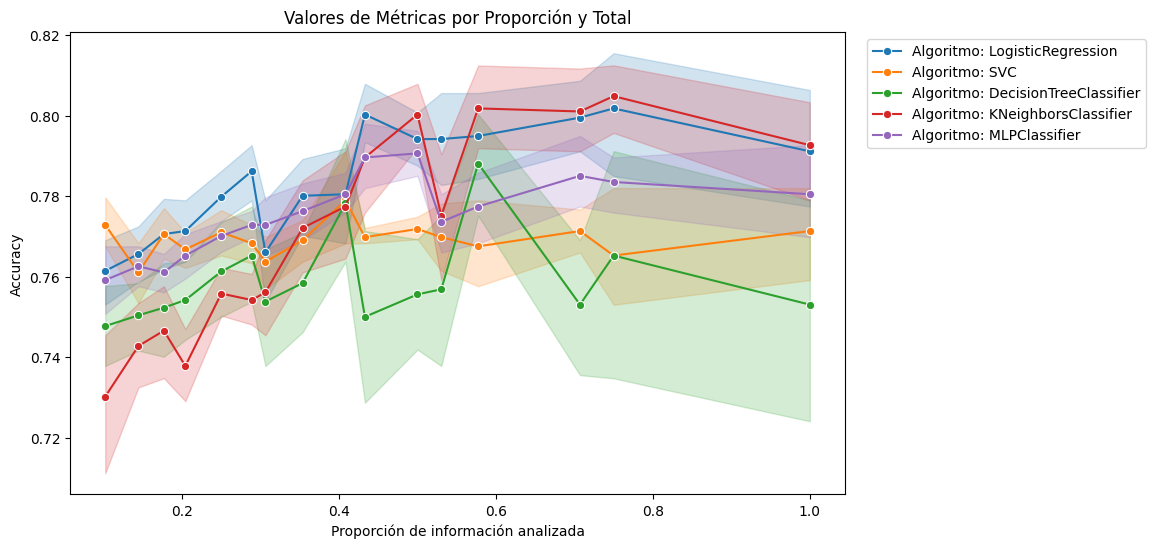
\includegraphics[width=0.6\linewidth]{figs/cap7/figura_13}
	\caption{Eficacia de los algoritmos de aprendizaje supervisado en función del índice de cantidad de información}
	\label{fig:figura207}
\end{figure}
	
	
\end{frame}


\subsection{ Objetivos 2 y 3: Tipo de bloques temporales}
%%========= Diapositiva con ítems resaltados con colores:
\begin{frame}
	\frametitle{Resultados. Objetivos 2 y 3: Tipo de bloques temporales}
	\begin{block}{Analizar la eficacia de las predicciones utilizando
			distintos tipos de subdivisión en bloques temporales: secuenciales vs encadenados.}
		Índice de amplitud o cobertura de la información.
	\end{block}
	
\begin{figure}[H]
	\centering
	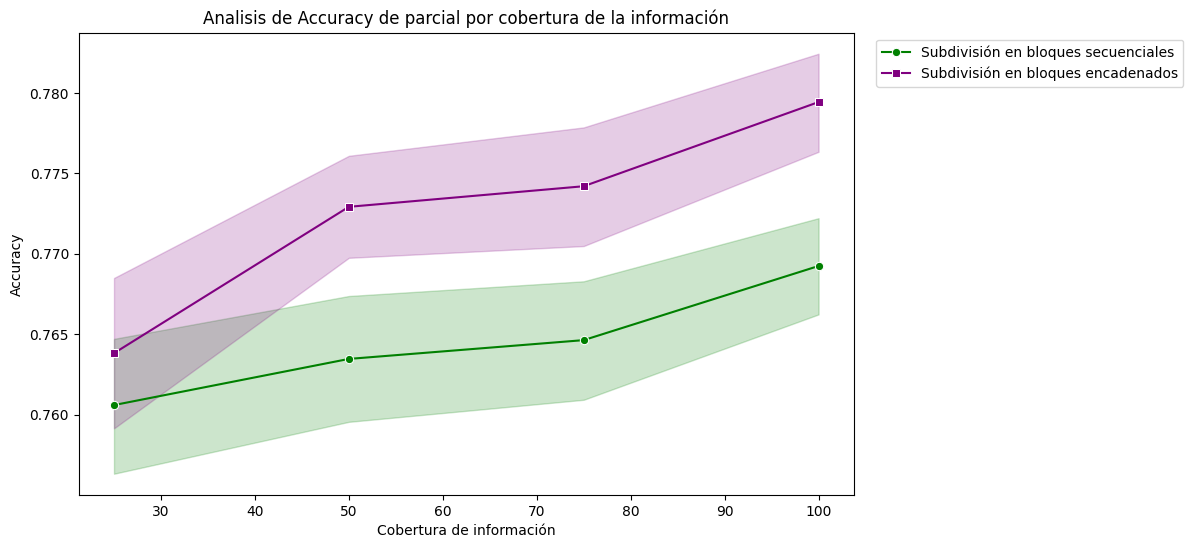
\includegraphics[width=0.7\linewidth]{figs/cap7/figura_15}
	\caption{Eficacia de los tipos de bloques temporales en función  de la cobertura temporal}
	
	\label{fig:figura212}
\end{figure}

\end{frame}


%========= Diapositiva con ítems resaltados con colores:
\begin{frame}
	\frametitle{Resultados. Objetivos 2 y 3: Tipo de bloques temporales}
\begin{block}{Analizar la eficacia de las predicciones utilizando
		distintos tipos de subdivisión en bloques temporales: secuenciales vs encadenados.}
		Índice de tamaño de la unidad de información.
	\end{block}
	
\begin{figure}[H]
	\centering
	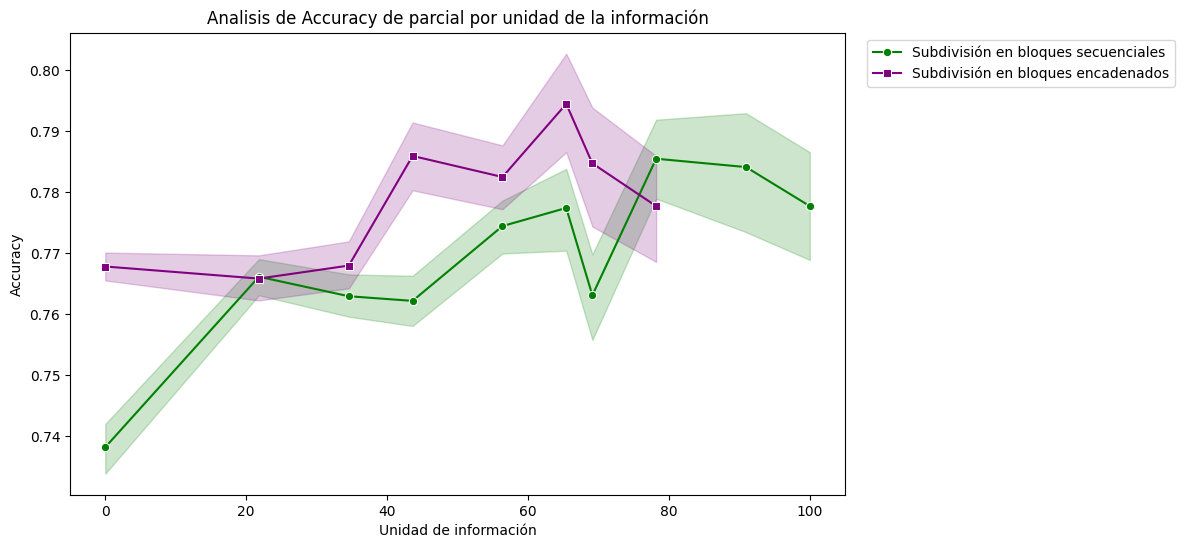
\includegraphics[width=0.7\linewidth]{figs/cap7/figura_16}
	\caption{Eficacia de los tipos de bloques temporales en función del índice de unidad de información}
	
	\label{fig:figura213}
\end{figure}

	
\end{frame}


%========= Diapositiva con ítems resaltados con colores:
\begin{frame}
	\frametitle{Resultados. Objetivos 2 y 3: Tipo de bloques temporales}
\begin{block}{Analizar la eficacia de las predicciones utilizando
		distintos tipos de subdivisión en bloques temporales: secuenciales vs encadenados.}
		Índice de cantidad de información.
	\end{block}
	

\begin{figure}[H]
	\centering
	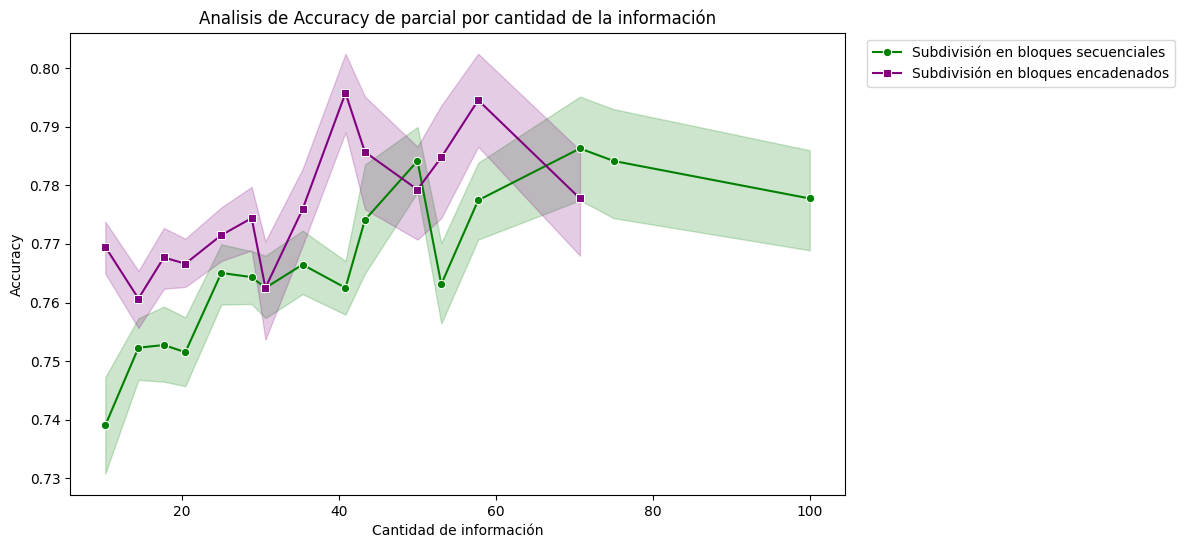
\includegraphics[width=0.7\linewidth]{figs/cap7/figura_17}
	\caption{Eficacia de los tipos de bloques temporales en función del índice de cantidad de información}
	\label{fig:figura214}
\end{figure}
	
\end{frame}



%========= Diapositiva con ítems resaltados con colores:
\begin{frame}
	\frametitle{Resultados. Objetivos 2 y  3: Tipo de bloques temporales}
\begin{block}{Analizar la eficacia de las predicciones utilizando
		distintos tipos de subdivisión en bloques temporales: secuenciales vs encadenados.}

	Evaluación conjunta de la cobertura y la unidad de información.
	\end{block}	
\begin{figure}[H]
	\centering
	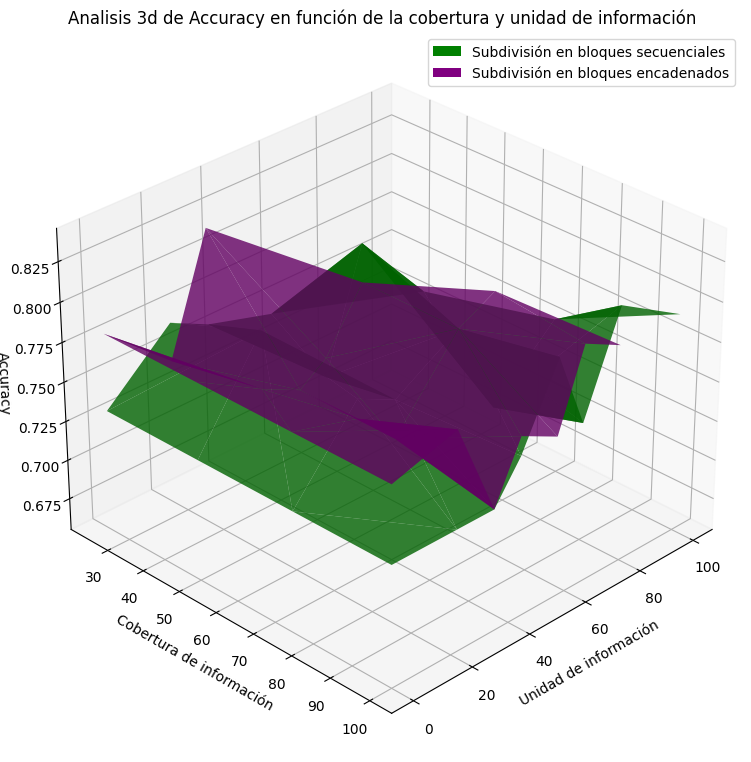
\includegraphics[width=0.45\linewidth]{figs/cap7/figura_18}
	\caption{Rendimiento de la métrica de eficacia de Accuracy en función de la cobertura y la unidad de información}
	
	\label{fig:figura215}
\end{figure}

	
\end{frame}


\subsection{Subobjetivo 1: Hipótesis del Capital Social Cognitivo}
%%========= Diapositiva con ítems resaltados con colores:
\begin{frame}
	\frametitle{Resultados. Subobjetivo 1: Hipótesis del Capital Social Cognitivo (medidas ponderadas)}
	\begin{block}{Analizar la eficacia de las predicciones utilizando
			distintos tipos de medidas centrales: sin pesos vs con pesos.}
		Índice de amplitud o cobertura de la información.
	\end{block}
\begin{figure}[H]
	\centering
	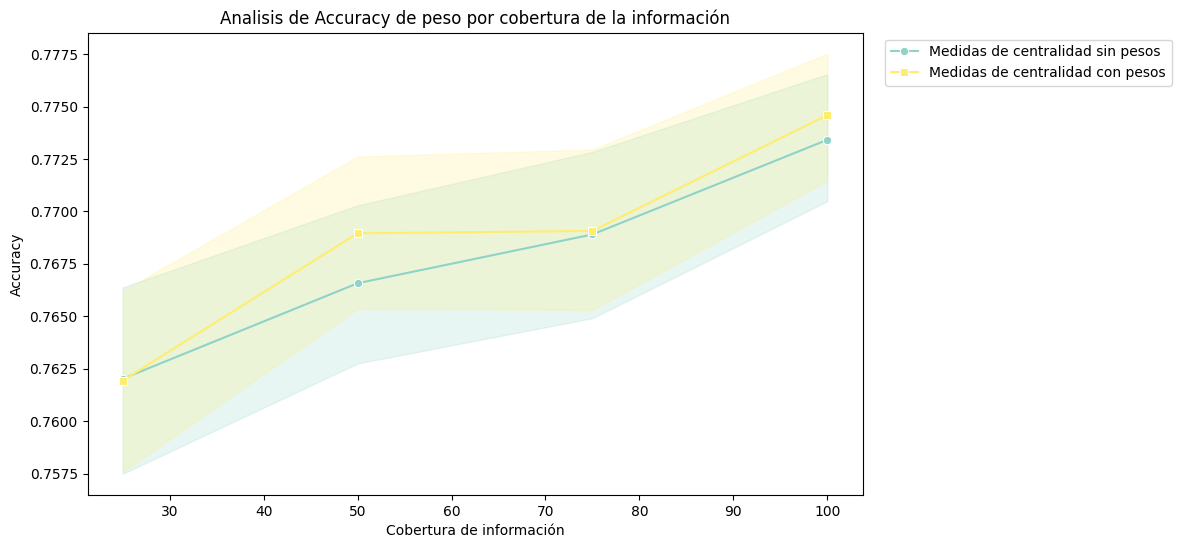
\includegraphics[width=0.6\linewidth]{figs/cap7/figura_34}
	\caption{Eficacia de los tipos de medidas de centralidad en función de la amplitud de información}
	
	\label{fig:figura218}
\end{figure}


	
\end{frame}


%========= Diapositiva con ítems resaltados con colores:
\begin{frame}
	\frametitle{Resultados. Subobjetivo 1: Hipótesis del Capital Social Cognitivo (medidas ponderadas)}
	\begin{block}{Analizar la eficacia de las predicciones utilizando
		distintos tipos de medidas centrales: sin pesos vs con pesos.}
		Índice de tamaño de la unidad de información.
	\end{block}
	
\begin{figure}[H]
	\centering
	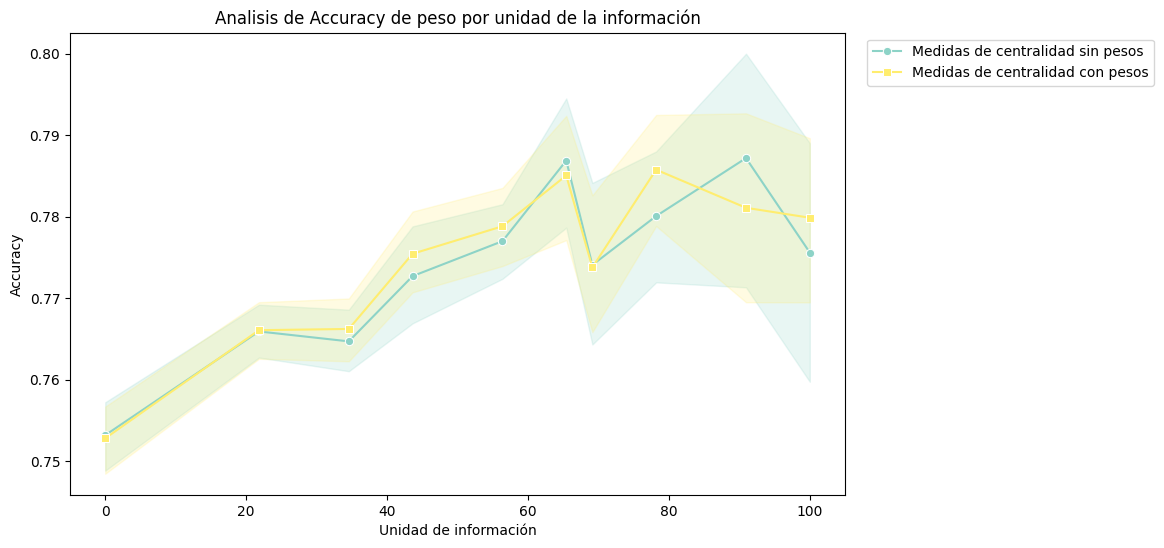
\includegraphics[width=0.6\linewidth]{figs/cap7/figura_35}
	\caption{Eficacia de los tipos de medidas de centralidad en función del índice de unidad de información}
	
	\label{fig:figura219}
\end{figure}

	
	
\end{frame}


%========= Diapositiva con ítems resaltados con colores:
\begin{frame}
	\frametitle{Resultados. Subobjetivo 1: Hipótesis del Capital Social Cognitivo (medidas ponderadas)}
	\begin{block}{Analizar la eficacia de las predicciones utilizando
		distintos tipos de medidas centrales: sin pesos vs con pesos.}
		Índice de cantidad de información.
	\end{block}
	

\begin{figure}[H]
	\centering
	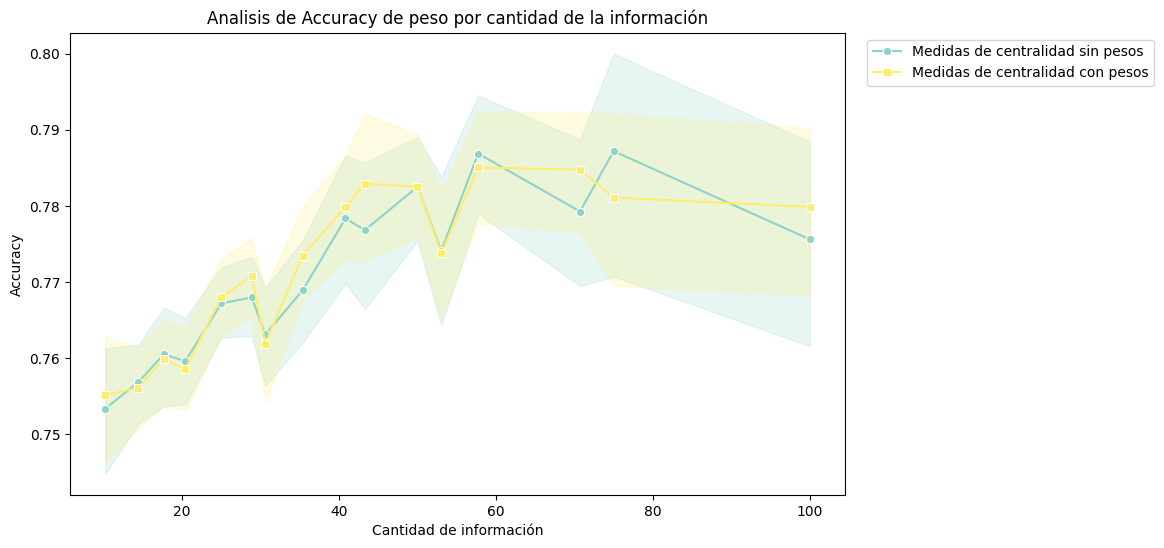
\includegraphics[width=0.6\linewidth]{figs/cap7/figura_36}
	\caption{Eficacia de los tipos de medidas de centralidad en función del índice de cantidad de información}
	\label{fig:figura220}
\end{figure}
	
\end{frame}



%========= Diapositiva con ítems resaltados con colores:
\begin{frame}
	\frametitle{Resultados. Subobjetivo 1: Hipótesis del Capital Social Cognitivo (medidas ponderadas)}
	\begin{block}{Analizar la eficacia de las predicciones utilizando
		distintos tipos de medidas centrales: sin pesos vs con pesos.}
		

	Evaluación conjunta de la cobertura y la unidad de información.
	\end{block}	
\begin{figure}[H]
	\centering
	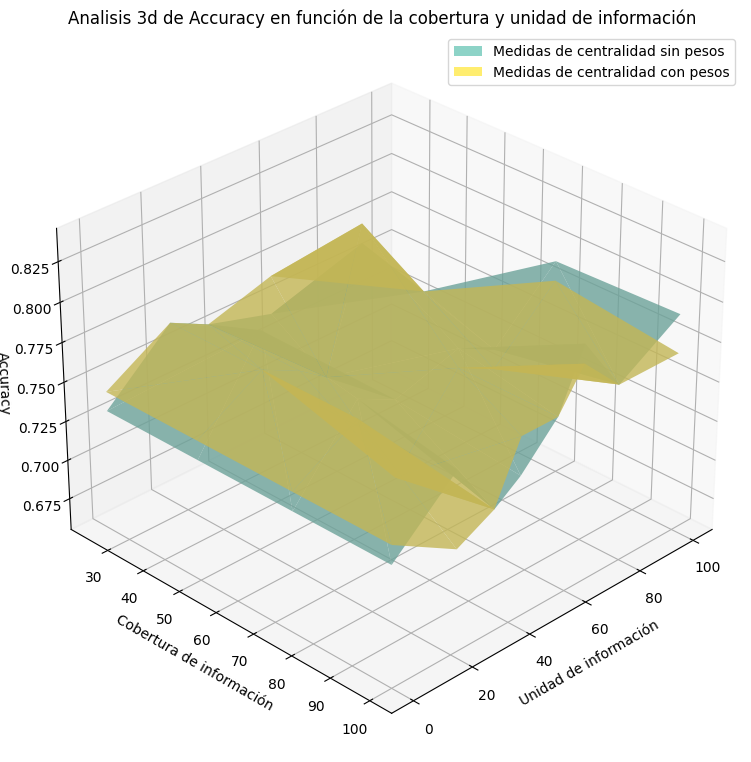
\includegraphics[width=0.45\linewidth]{figs/cap7/figura_37}
	\caption{Rendimiento de la métrica de eficacia de Accuracy en función de la cobertura y la unidad de información}
	
	\label{fig:figura221}
\end{figure}
	
	
\end{frame}





\subsection{Subobjetivo 2: Hipótesis del Esquema Social Cognitivo}
%%========= Diapositiva con ítems resaltados con colores:
\begin{frame}
	\frametitle{Resultados. Subobjetivo 2: Hipótesis del Esquema Social Cognitivo (medidas globales)}
\begin{block}{Analizar la eficacia de las predicciones utilizando
		distintos tipos de medidas centrales: locales vs globales (híbridas).}
		Índice de amplitud o cobertura de la información.
	\end{block}
\begin{figure}[H]
	\centering
	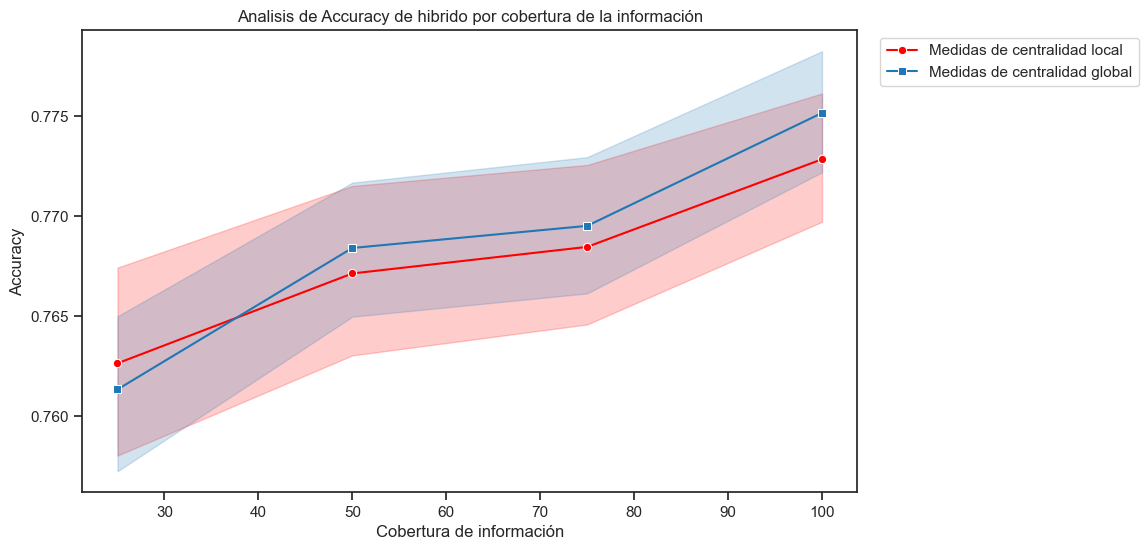
\includegraphics[width=0.6\linewidth]{figs/cap7/figura_43}
	\caption{Eficacia de los tipos de medidas de centralidad en función del porcentaje de cobertura temporal o amplitud de la información}
	
	\label{fig:figura224}
\end{figure}

\end{frame}


%========= Diapositiva con ítems resaltados con colores:
\begin{frame}
	\frametitle{Resultados. Subobjetivo 2: Hipótesis del Esquema Social Cognitivo (medidas globales)}
\begin{block}{Analizar la eficacia de las predicciones utilizando
		distintos tipos de medidas centrales: locales vs globales (híbridas).}
		Índice de tamaño de la unidad de información.
	\end{block}
	
\begin{figure}[H]
	\centering
	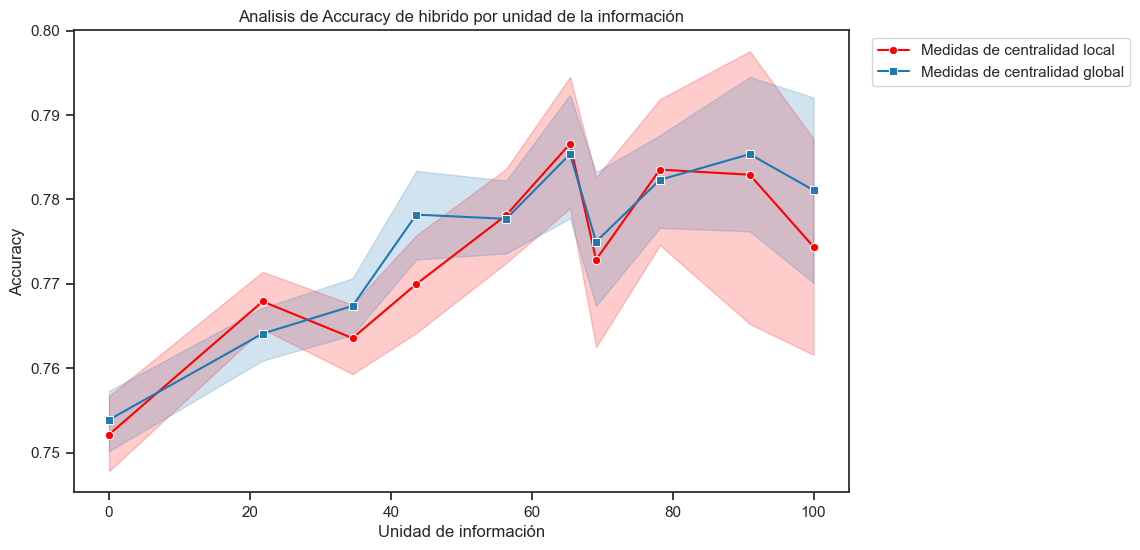
\includegraphics[width=0.6\linewidth]{figs/cap7/figura_44}
	\caption{Eficacia de los tipos de medidas de centralidad en función de la unidad  de información}
	\label{fig:figura225}
\end{figure}

	
	
	
\end{frame}


%========= Diapositiva con ítems resaltados con colores:
\begin{frame}
	\frametitle{Resultados. Subobjetivo 2: Hipótesis del Esquema Social Cognitivo (medidas globales)}
\begin{block}{Analizar la eficacia de las predicciones utilizando
		distintos tipos de medidas centrales: locales vs globales (híbridas).}
		Índice de cantidad de información.
	\end{block}
	
\begin{figure}[H]
	\centering
	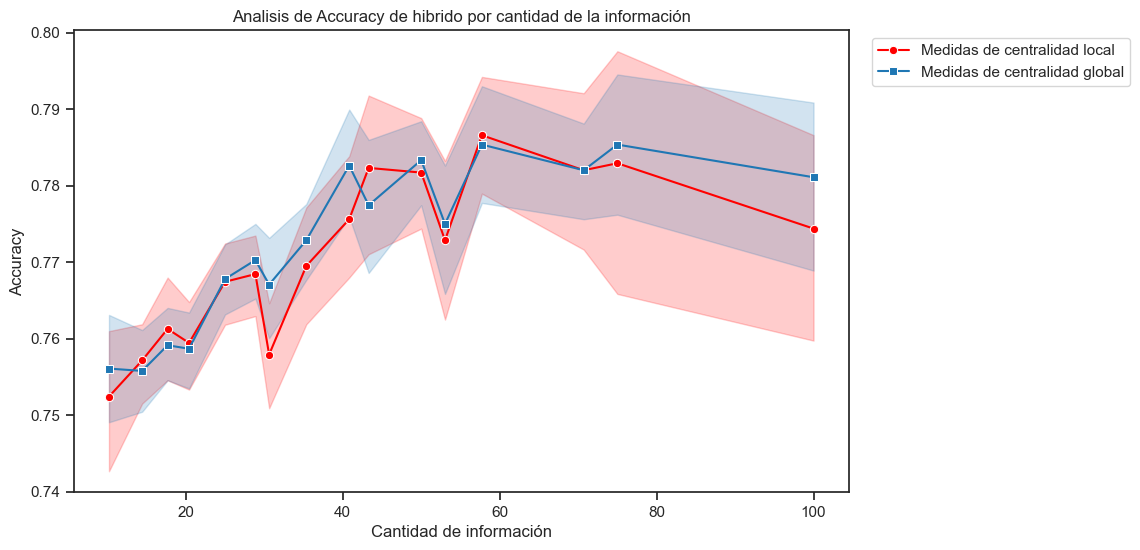
\includegraphics[width=0.6\linewidth]{figs/cap7/figura_45}
	\caption{Eficacia de los tipos de medidas de centralidad en función de la calidad  de información}
	\label{fig:figura226}
\end{figure}


	
	
	
\end{frame}



%========= Diapositiva con ítems resaltados con colores:
\begin{frame}
	\frametitle{Resultados. Subobjetivo 2: Hipótesis del Esquema Social Cognitivo (medidas globales)}
\begin{block}{Analizar la eficacia de las predicciones utilizando
		distintos tipos de medidas centrales: locales vs globales (híbridas).}
		

	Evaluación conjunta de la cobertura y la unidad de información.
		\end{block}

\begin{figure}[H]
	\centering
	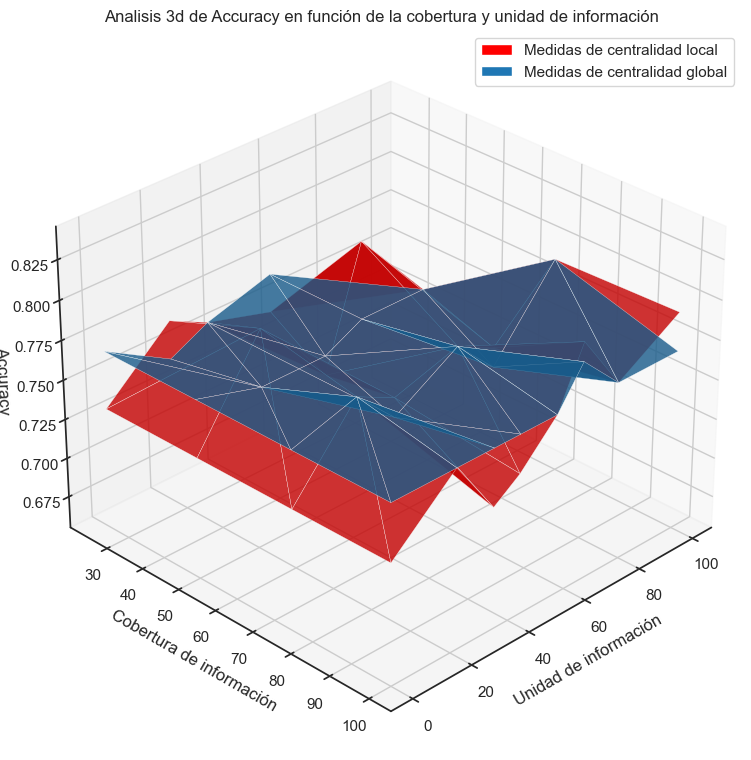
\includegraphics[width=0.45\linewidth]{figs/cap7/figura_46}
	\caption{Rendimiento de la métrica de eficacia de Accuracy en función de la cobertura y la unidad de información}
	
	\label{fig:figura227}
\end{figure}
	
\end{frame}






\subsection{Subobjetivo 3: Hipótesis del Balance Social Cognitivo}
%%========= Diapositiva con ítems resaltados con colores:
\begin{frame}
	\frametitle{Resultados. Subobjetivo 3: Hipótesis del Balance Social Cognitivo (medidas centrales y medidas de emoción)}
	\begin{block}{Analizar la eficacia de las predicciones utilizando
			medidas centrales vs medidas centrales y de sentimentos.}
		Índice de amplitud o cobertura de la información.
	\end{block}
\begin{figure}[H]
	\centering
	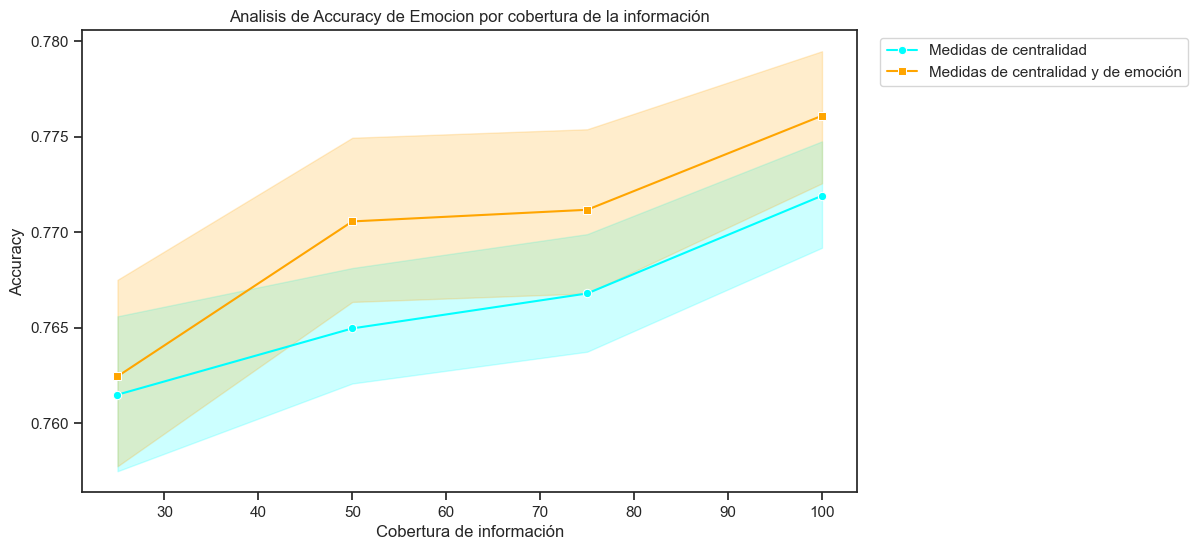
\includegraphics[width=0.6\linewidth]{figs/cap7/figura_53}
	\caption{Eficacia del uso de medidas de centralidad sin o con medidas de sentimiento en función del porcentaje de cobertura temporal o amplitud de la información}
	
	\label{fig:figura229}
\end{figure}

	
	
\end{frame}


%========= Diapositiva con ítems resaltados con colores:
\begin{frame}
	\frametitle{Resultados. Subobjetivo 3: Hipótesis del Balance Social Cognitivo (medidas centrales y medidas de emoción)}
\begin{block}{Analizar la eficacia de las predicciones utilizando
		medidas centrales vs medidas centrales y de sentimentos.}
		Índice de tamaño de la unidad de información.
	\end{block}
	
\begin{figure}[H]
	\centering
	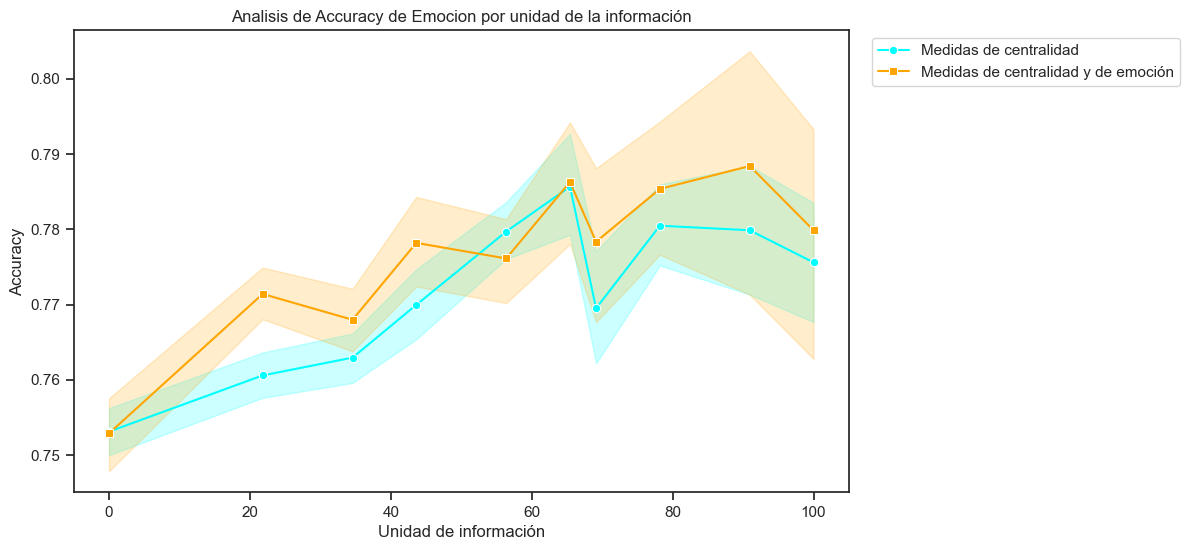
\includegraphics[width=0.6\linewidth]{figs/cap7/figura_54}
	\caption{Eficacia del uso de medidas de centralidad sin o con medidas de sentimiento en función del índice de unidad de información}
	
	\label{fig:figura230}
\end{figure}
	
	
	
\end{frame}


%========= Diapositiva con ítems resaltados con colores:
\begin{frame}
	\frametitle{Resultados. Subobjetivo 3: Hipótesis del Balance Social Cognitivo (medidas centrales y medidas de emoción)}
\begin{block}{Analizar la eficacia de las predicciones utilizando
		medidas centrales vs medidas centrales y de sentimentos.}
		Índice de cantidad de información.
	\end{block}
	
	
\begin{figure}[H]
	\centering
	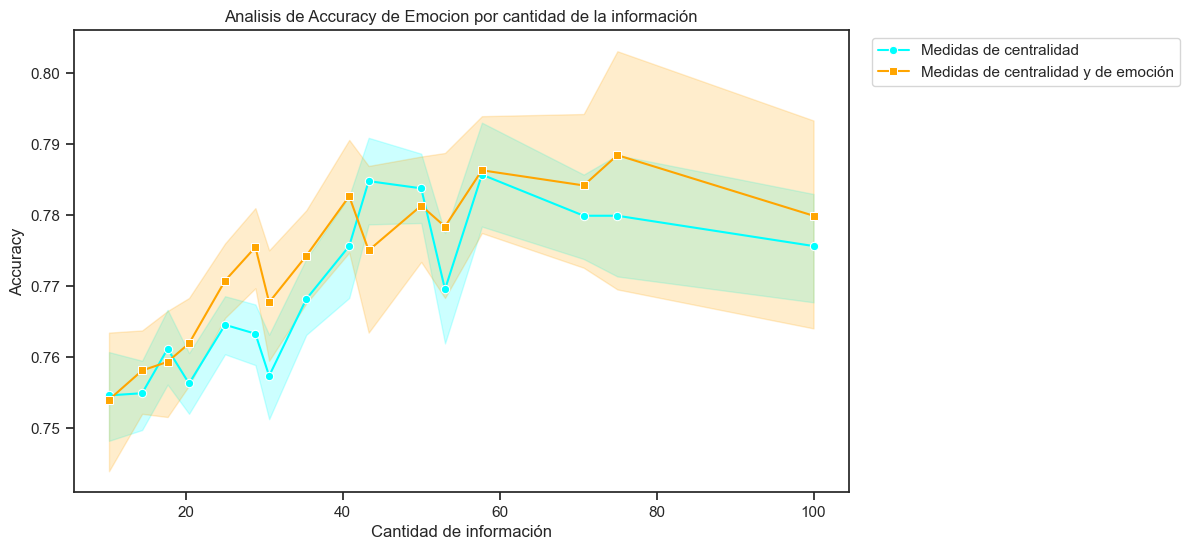
\includegraphics[width=0.6\linewidth]{figs/cap7/figura_55}
	\caption{Eficacia del uso de medidas de centralidad sin o con medidas de sentimiento en función del índice de cantidad de información}
	\label{fig:figura231}
\end{figure}

	
	
	
\end{frame}



%========= Diapositiva con ítems resaltados con colores:
\begin{frame}
	\frametitle{Resultados. Subobjetivo 3: Hipótesis del Balance Social Cognitivo (medidas centrales y medidas de emoción)}
\begin{block}{Analizar la eficacia de las predicciones utilizando
		medidas centrales vs medidas centrales y de sentimentos.}
		

	Evaluación conjunta de la cobertura y la unidad de información.
	\end{block}	
\begin{figure}[H]
	\centering
	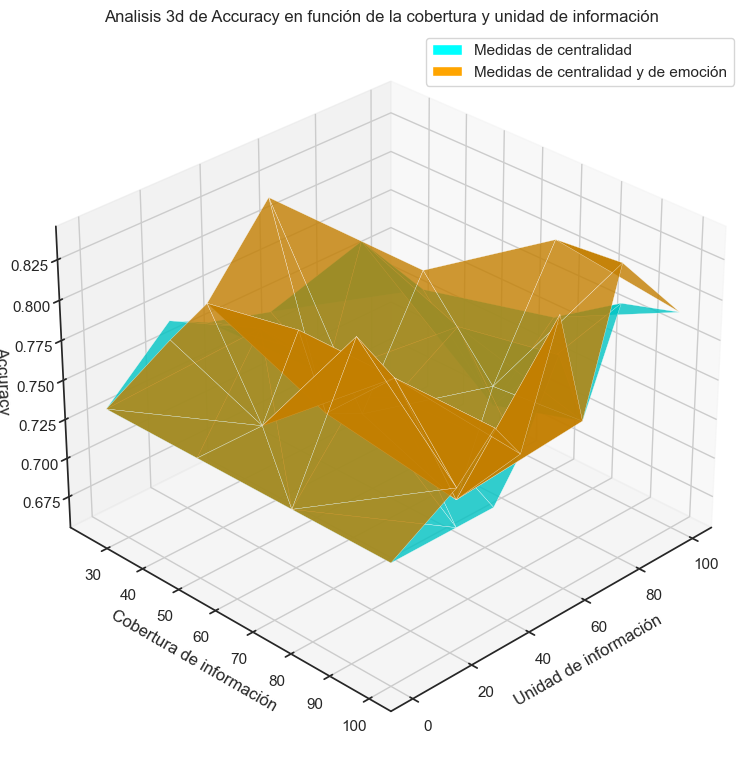
\includegraphics[width=0.45\linewidth]{figs/cap7/figura_56}
	\caption{Rendimiento de la métrica de eficacia de Accuracy en función de la cobertura y la unidad de información}
	
	\label{fig:figura233}
\end{figure}
	
\end{frame}



\section{Conclusiones}
\begin{frame}
	\frametitle{Resultados clave}
  \begin{itemize}
	\item A medida que aumenta el porcentaje de cobertura temporal, la eficacia de todos los tipos de subdivisión en bloques también incrementa.
	
	\item Existe un equilibrio entre la cantidad (amplitud x unidad) de información analizada y la capacidad predictiva del modelo, ya que el punto máximo de eficacia en la predicción no se encuentra en el máximo nivel de cobertura temporal.
	
	\item La subdivisión del análisis de la red social en bloques temporales encadenados muestra una eficacia superior en comparación con la subdivisión en bloques secuenciales.
	
	\item Las medidas de centralidad globales que evalúan la posición en la red de los nodos vecinos pueden ser más eficaces para capturar la estructura de la red del estudiante y predecir su abandono de la asignatura.
	
	\item La integración de medidas emocionales con las medidas de centralidad mejora la capacidad predictiva del modelo.

\end{itemize}
\end{frame}



\begin{frame}
	\frametitle{Limitaciones y futuras investigaciones}
	
	\begin{itemize}
		\item Tamaño limitado y sesgado de los datos analizados.
		\item Uso de medidas de cohesión de la red y algoritmos de detección de comunidades diferentes.
		\item Integración de medidas de centralidad y análisis de sentimiento para comprender la relación entre emociones y posición de los nodos.
		\item Utilización de técnicas de balanceo de datos, como SMOTE, para abordar el desbalance de los datos.
		\item Evaluación de la importancia relativa de las características mediante la técnica SHAP.
		\item Implementación de técnicas de ensamblaje, como Bagging o RandomForest.
	\end{itemize}
\end{frame}



\begin{frame}
	\frametitle{Aplicación de los resultados}
	
	\begin{enumerate}
		\item Identificación temprana de estudiantes en riesgo: El análisis de la interacción en los foros de las asignaturas, considerando medidas de centralidad y evaluaciones emocionales, puede ayudar a identificar a los estudiantes que están en riesgo de abandonar la asignatura o que están experimentando dificultades académicas.
		
		\item Diseño de estrategias de enseñanza personalizadas: La comprensión de los patrones de comportamiento y las preferencias de los estudiantes en los foros de la asignatura puede guiar el diseño de estrategias de enseñanza personalizadas.
		
		\item Mejora de la experiencia del estudiante en entornos de aprendizaje en línea: El análisis de medidas de centralidad y evaluaciones emocionales en los foros de las asignaturas puede proporcionar información valiosa para mejorar la experiencia del estudiante en entornos virtuales.
		
		\item Desarrollo de sistemas de recomendación personalizados: La combinación de medidas de centralidad y emocionales puede ser utilizada para desarrollar sistemas de recomendación personalizados.
	\end{enumerate}
\end{frame}


\begin{frame}[plain]
\large{\titlepage}
\note[item]{Y hasta aquí mi exposición.}
\note[item]{Quedo a disposición del tribunal...}
\end{frame}



%%%
% CONTENIDO. BIBLIOGRAFÍA.
%%%%
%\nocite{*} %incluye TODOS los documentos de la base de datos bibliográfica sean o no citados en el texto
\bibliography{bibliografia/bibliografia} % Archivo que contiene la bibliografía
%\bibliographystyle{apacite}
\bibliographystyle{IEEEtranN}
%\bibliographystyle{amsplain}

\end{document}
